\chapter{The OpenMC Monte Carlo Code}
\label{chap:openmc}

\section{Background}

As part of the present work, a general Monte Carlo neutron transport code was
written from scratch with an emphasis on high performance algorithms, accurate
physics capabilities, and modern software design practices. The development of
the code started as a simplistic platform, first mentioned in
\cite{lanl-romano-2009}, within which algorithms could be easily tested. At that
stage, the geometry was limited to a simple structured mesh and all physics were
based on predefined fictitious multigroup cross sections. However, as further
studies of domain and data decomposition schemes, described in
\autoref{chap:domain-decomp} and \autoref{chap:data-decomp}, demanded that
realistic geometry and physics be present, a decision was made to greatly expand
the capabilities of the code.

In early 2011, the geometry and physics from the original structured-mesh,
multigroup code was gutted and replaced with constructive solid geometry
routines and physics based on continuous-energy cross sections. In Fall 2011,
the input file format was changed to an XML format and a basic outline of the
current tally system was introduced. Since then, improvements have been made in
physics methods, geometry capabilities, and input/output options.

OpenMC has been described in a recent paper in \emph{Annals of Nuclear Energy}
\cite{ane-romano-2013}. Further developments will be reported in a paper at the
M\&C 2013 conference \cite{mc-romano-2013}.

\section{Overview of Program Flow}

OpenMC performs a Monte Carlo simulation one particle at a time --- at no point
is more than one particle being tracked on a single program
instance\footnote{When executed in parallel, each program instance tracks one
  particle at a time.}. Before any particles are tracked, the problem must be
initialized. This involves the following steps:
\begin{itemize}
\item Read input files and build data structures for the geometry, materials,
  tallies, and other associated variables.
\item Initialize the pseudorandom number generator.
\item Read ACE format cross sections specified in the problem.
\item If using a special energy grid treatment such as a union energy grid with
  pointers, that must be initialized as well.
\item In a fixed source problem, source sites are sampled from the specified
  source. In an eigenvalue problem, source sites are sampled from some initial
  source distribution or from a source file. The source sites consist of
  coordinates, a direction, and an energy.
\end{itemize}
Once initialization is complete, the actual transport simulation can
proceed. The life of a single particle will proceed as follows:
\begin{enumerate}
\item The particle's properties are initialized from a source site previously
  sampled.
\item Based on the particle's coordinates, the current cell in which the
  particle resides is determined.
\item The energy-dependent cross sections for the material that the particle is
  currently in are determined. Note that this includes the total cross section,
  which is not pre-calculated.
\item The distance to the nearest boundary of the particle's cell is determined
  based on the bounding surfaces to the cell.
\item The distance to the next collision is sampled. If the total material
  cross section is $\Sigma_t$, this can be shown to be
  \begin{equation}
    d = -\frac{\ln \xi}{\Sigma_t}
  \end{equation}
  where $\xi$ is a pseudorandom number sampled from a uniform distribution on
  $[0,1)$.
\item If the distance to the nearest boundary is less than the distance to the
  next collision, the particle is moved forward to this boundary. Then, the
  process is repeated from step 2. If the distance to collision is closer than
  the distance to the nearest boundary, then the particle will undergo a
  collision.
\item The material at the collision site may consist of multiple
  nuclides. First, the nuclide with which the collision will happen is sampled
  based on the total cross sections. If the total cross section of material $i$
  is $\Sigma_{t,i}$, then the probability that any nuclide is sampled is
  \begin{equation}
    P(i) = \frac{\Sigma_{t,i}}{\Sigma_t}.
  \end{equation}
\item Once the specific nuclide is sampled, a reaction for that nuclide is
  randomly sampled based on the microscopic cross sections. If the microscopic
  cross section for some reaction $x$ is $\sigma_x$ and the total microscopic
  cross section for the nuclide is $\sigma_t$, then the probability that
  reaction $x$ will occur is
  \begin{equation}
    P(x) = \frac{\sigma_x}{\sigma_t}.
  \end{equation}
\item If the sampled reaction is elastic or inelastic scattering, the outgoing
  energy and angle is sampled from the appropriate distribution.  Reactions of
  type $(n,xn)$ are treated as scattering and the weight of the particle is
  increased by the multiplicity of the reaction. The particle then continues
  from step 3. If the reaction is absorption or fission, the particle dies and
  if necessary, fission sites are created and stored in the fission bank.
\end{enumerate}
After all particles have been simulated, there are a few final tasks that must
be performed before the run is finished. This include the following:
\begin{itemize}
\item With the accumulated sum and sum of squares for each tally, the sample
  mean and its variance is calculated.
\item All tallies and other results are written to disk.
\item If requested, a source file is written to disk
\item All allocatable arrays are deallocated.
\end{itemize}

\section{Geometry}

\subsection{Constructive Solid Geometry}

OpenMC uses a technique known as constructive solid geometry (CSG) to build
arbitrarily complex three-dimensional models in Euclidean space. In a CSG model,
every unique object is described as the union, intersection, or difference of
\emph{half-spaces} created by bounding surfaces. Every surface divides all of
space into exactly two half-spaces. We can mathematically define a surface as a
collection of points that satisfy an equation of the form $f(x,y,z) = 0$ where
$f(x,y,z)$ is a given function. All coordinates for which $f(x,y,z) < 0$ are
referred to as the negative half-space (or simply the \emph{negative side}) and
coordinates for which $f(x,y,z) > 0$ are referred to as the positive half-space.

Let us take the example of a sphere centered at the point $(x_0,y_0,z_0)$
with radius $R$. One would normally write the equation of the sphere as
\begin{equation}
  \label{eq:sphere-equation}
  (x - x_0)^2 + (y - y_0)^2 + (z - z_0)^2 = R^2.
\end{equation}
By subtracting the right-hand term from both sides of
\eqref{eq:sphere-equation}, we can then write the surface equation for the
sphere:
\begin{equation}
  \label{eq:surface-equation-sphere}
  f(x,y,z) = (x - x_0)^2 + (y - y_0)^2 + (z - z_0)^2 - R^2 = 0
\end{equation}
One can confirm that any point inside this sphere will correspond to
$f(x,y,z) < 0$ and any point outside the sphere will correspond to
$f(x,y,z) > 0$.

In OpenMC, every surface defined by the user is assigned an integer to uniquely
identify it. We can then refer to either of the two half-spaces created by a
surface by a combination of the unique ID of the surface and a positive/negative
sign. \autoref{fig:halfspace} shows an example of an ellipse with unique ID 1
dividing space into two half-spaces.
\begin{figure}[htb]
  \centering
  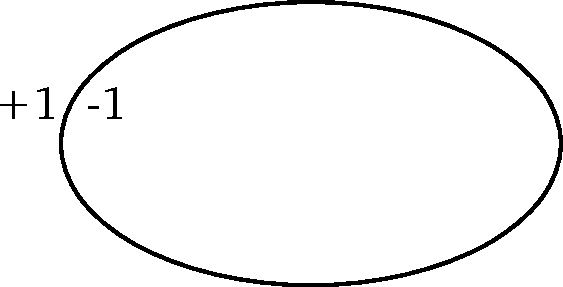
\includegraphics[width=3.0in]{figures/ch2/halfspace.pdf}
  \caption{Example of an ellipse and its associated half-spaces.}
  \label{fig:halfspace}
\end{figure}

References to half-spaces created by surfaces are used to define regions of
space of uniform composition, known as \emph{cells}. While some codes allow
regions to be defined by intersections, unions, and differences or half-spaces,
OpenMC is currently limited to cells defined only as intersections of
half-spaces. Thus, the specification of the cell must include a list of
half-space references whose intersection defines the region. The region is then
assigned a material defined elsewhere. \autoref{fig:union} shows an example of a
cell defined as the intersection of an ellipse and two planes.
\begin{figure}[htb]
  \centering
  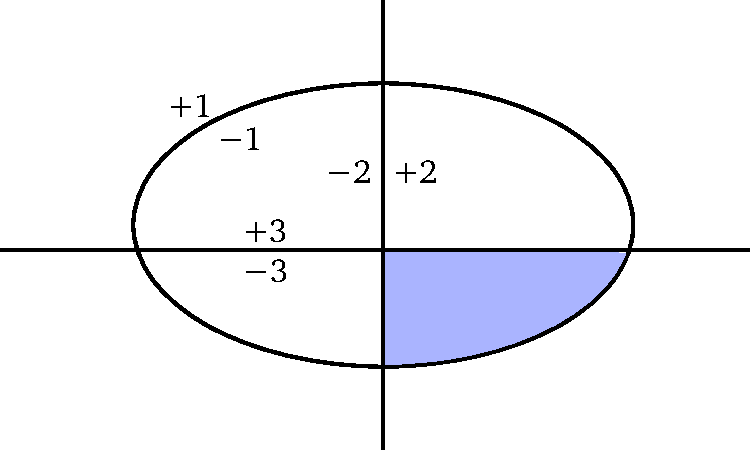
\includegraphics[width=4.0in]{figures/ch2/union.pdf}
  \caption{The shaded region represents a cell bounded by three surfaces.}
  \label{fig:union}
\end{figure}

The ability to form regions based on bounding quadratic surfaces enables OpenMC
to model arbitrarily complex three-dimensional objects. In practice, one is
limited only by the different surface types available in
OpenMC. \autoref{tab:surfaces} lists the available surface types, the identifier
used to specify them in input files, the corresponding surface equation, and the
input parameters needed to fully define the surface.
\begin{table}[htb]
  \caption{Surface types available in OpenMC.}
  \label{tab:surfaces}
  \footnotesize{
  \begin{tabular}{c c c c}
    \toprule
    Surface & Identifier & Equation & Parameters \\
    \midrule
    Plane perpendicular to $x$-axis & x-plane & $x - x_0 = 0$ & $x_0$ \\

    Plane perpendicular to $y$-axis & y-plane & $y - y_0 = 0$ & $y_0$ \\

    Plane perpendicular to $z$-axis & z-plane & $z - z_0 = 0$ & $z_0$ \\

    Arbitrary plane & plane & $Ax + By + Cy = D$ & $A \; B \; C \; D$ \\

    Infinite cylinder parallel to $x$-axis & x-cylinder & $(y - y_0)^2 + (z -
    z_0)^2 = R^2$ & $y_0 \; z_0 \; R$ \\

    Infinite cylinder parallel to $y$-axis & y-cylinder & $(x - x_0)^2 + (z -
    z_0)^2 = R^2$ & $x_0 \; z_0 \; R$ \\

    Infinite cylinder parallel to $z$-axis & z-cylinder & $(x - x_0)^2 + (y -
    y_0)^2 = R^2$ & $x_0 \; y_0 \; R$ \\

    Sphere & sphere & $(x - x_0)^2 + (y - y_0)^2 + (z - z_0)^2 = R^2$ & $x_0 \;
    y_0 \; z_0 \; R$ \\

    Cone parallel to the $x$-axis & x-cone & $(y - y_0)^2 + (z - z_0)^2 = R^2(x
    - x_0)^2 $ & $x_0 \; y_0 \; z_0 \; R^2$ \\

    Cone parallel to the $y$-axis & y-cone & $(x - x_0)^2 + (z - z_0)^2 = R^2(y
    - y_0)^2 $ & $x_0 \; y_0 \; z_0 \; R^2$ \\

    Cone parallel to the $z$-axis & z-cone & $(x - x_0)^2 + (y - y_0)^2 = R^2(z
    - z_0)^2 $ & $x_0 \; y_0 \; z_0 \; R^2$ \\

    \bottomrule
  \end{tabular}
  }
\end{table}

\subsubsection{Universes}

OpenMC supports universe-based geometry similar to the likes of MCNP
\cite{lanl-x5-2008} and Serpent \cite{vtt-leppanen-2007}. This capability
enables users to model any identical repeated structures once and then fill them
in various spots in the geometry. A prototypical example of a repeated structure
would be a fuel pin within a fuel assembly or a fuel assembly within a core.

Each cell in OpenMC can either be filled with a normal material or with a
universe. If the cell is filled with a universe, only the region of the universe
that is within the defined boundaries of the parent cell will be present in the
geometry. That is to say, even though a collection of cells in a universe may
extend to infinity, not all of the universe will be ``visible'' in the geometry
since it will be truncated by the boundaries of the cell that contains it.

When a cell is filled with a universe, it is possible to specify that the
universe filling the cell should be rotated and translated. This is done through
the \texttt{rotation} and \texttt{translation} attributes on a cell (note though
that these can only be specified on a cell that is filled with a universe, not a
material).

It is not necessary to use or assign universes in a geometry if there are no
repeated structures. Any cell in the geometry that is not assigned to a
specified universe is automatically part of the \emph{base universe} whose
coordinates are just the normal coordinates in Euclidean space.

\subsubsection{Lattices}

Often times, repeated structures in a geometry occur in a regular pattern such
as a rectangular or hexagonal lattice. In such a case, it would be cumbersome
for a user to have to define the boundaries of each of the cells to be filled
with a universe. Thus, OpenMC provides a lattice capability similar to that used
in MCNP and Serpent.

The implementation of lattices is similar in principle to universes --- instead
of a cell being filled with a universe, the user can specify that it is filled
with a finite lattice. The lattice is then defined by a two-dimensional array of
universes that are to fill each position in the lattice. A good example of the
use of lattices and universes can be seen in the OpenMC model for the Monte
Carlo Performance benchmark \cite{romano-2012}.

\subsection{Computing the Distance to Nearest Boundary}

One of the most basic algorithms in any Monte Carlo code is determining the
distance to the nearest surface within a cell. Since each cell is defined by
the surfaces that bound it, if we compute the distance to all surfaces bounding
a cell, we can determine the nearest one.

With the possibility of a particle having coordinates on multiple levels
(universes) in a geometry, we must exercise care when calculating the distance
to the nearest surface. Each different level of geometry has a set of boundaries
with which the particle's direction of travel may intersect. Thus, it is
necessary to check the distance to the surfaces bounding the cell in each
level. This should be done starting at the highest (most global) level going
down to the lowest (most local) level. That ensures that if two surfaces on
different levels are coincident, by default the one on the higher level will be
selected as the nearest surface. Although they are not explicitly defined, it is
also necessary to check the distance to surfaces representing lattice boundaries
if a lattice exists on a given level.

The following procedure is used to calculate the distance to each bounding
surface. Suppose we have a particle at $(x_0,y_0,z_0)$ traveling in the
direction $u_0,v_0,w_0$. To find the distance $d$ to a surface $f(x,y,z) = 0$,
we need to solve the equation:
\begin{equation}
  \label{eq:dist-to-boundary-1}
  f(x_0 + du_0, y + dv_0, z + dw_0) = 0.
\end{equation}
Since $f(x,y,z)$ in general is quadratic in $x$, $y$, and $z$, this implies that
$f(x_0 + du_0, y + dv_0, z + dw_0)$ is quadratic in $d$. Thus we expect at most
two real solutions to \eqref{eq:dist-to-boundary-1}. If no solutions to
\eqref{eq:dist-to-boundary-1} exist or the only solutions are complex, then the
particle's direction of travel will not intersect the surface. If the solution
to \eqref{eq:dist-to-boundary-1} is negative, this means that the surface is
``behind'' the particle, i.e. if the particle continues traveling in its current
direction, it will not hit the surface.

Once a distance has been computed to a surface, we need to check if it is closer
than previously-computed distances to surfaces. Unfortunately, we cannot just
use the minimum function because some of the calculated distances, which should
be the same in theory (e.g. coincident surfaces), may be slightly different due
to the use of floating-point arithmetic. Consequently, we should first check for
floating-point equality of the current distance calculated and the minimum found
thus far. This is done by checking if
\begin{equation}
  \label{eq:fp-distance}
  \frac{| d - d_{min} |}{d_{min}} < \epsilon
\end{equation}
where $d$ is the distance to a surface just calculated, $d_{min}$ is
the minimum distance found thus far, and $\epsilon$ is a small number. In
OpenMC, this parameter is set to $\epsilon = 10^{-14}$ since all floating
calculations are done on 8-byte floating point numbers.

\subsection{Finding a Cell Given a Point}
\label{sec:find-cell}

Another basic algorithm is to determine which cell contains a given point in the
global coordinate system, i.e. if the particle's position is $(x,y,z)$, what
cell is it currently in. This is done in the following manner in OpenMC. With
the possibility of multiple levels of coordinates, we must perform a recursive
search for the cell. First, we start in the highest (most global) universe,
which we call the base universe, and loop over each cell within that
universe. For each cell, we check whether the specified point is inside the cell
using the algorithm described in \autoref{sec:cell-contains}. If the cell is
filled with a normal material, the search is done and we have identified the
cell containing the point. If the cell is filled with another universe, we then
search all cells within that universe to see if any of them contain the
specified point. If the cell is filled with a lattice, the position within the
lattice is determined, and then whatever universe fills that lattice position is
recursively searched. The search ends once a cell containing a normal material
is found that contains the specified point.

\subsection{Determining if a Coordinate is in a Cell}
\label{sec:cell-contains}

To determine which cell a particle is in given it's coordinates, we need to be
able to check whether a given cell contains a point. The algorithm for
determining if a cell contains a point is as follows. For each surface that
bounds a cell, we determine the particle's sense with respect to the surface. As
explained earlier, if we have a point $(x_0,y_0,z_0)$ and a surface $f(x,y,z) =
0$, the point is said to have negative sense if $f(x_0,y_0,z_0) < 0$ and
positive sense if $f(x_0,y_0,z_0) > 0$. If for all surfaces, the sense of the
particle with respect to the surface matches the specified sense that defines
the half-space within the cell, then the point is inside the cell. Note that
this algorithm works only for \emph{simple cells} defined as intersections of
half-spaces.

It may help to illustrate this algorithm using a simple example. Let's say we
have a cell defined as\footnote{The input file syntax is defined in detail in
  the OpenMC User's Guide \cite{romano-2012-doc}.}
\begin{lstlisting}[language=xml,frame=none]
<surface id="1" type="sphere"  coeffs="0 0 0 10" />
<surface id="2" type="x-plane" coeffs="-3" />
<surface id="3" type="y-plane" coeffs="2" />
<cell id="1" surfaces="-1 2 -3" />
\end{lstlisting}
This means that the cell is defined as the intersection of the negative half
space of a sphere, the positive half-space of an x-plane, and the negative
half-space of a y-plane. Said another way, any point inside this cell must
satisfy the following equations
\begin{equation}
  \label{eq:cell-contains-example}
  \begin{split}
    x^2 + y^2 + z^2 - 10^2 &< 0 \\
    x - (-3) &> 0 \\
    x - 2 &< 0
  \end{split}
\end{equation}
In order to determine if a point is inside the cell, we would substitute its
coordinates into \eqref{eq:cell-contains-example}. If the resulting inequalities
are satisfied, than the point is indeed inside the cell.

\subsection{Handling Surface Crossings}

A particle will cross a surface if the distance to the nearest surface is closer
than the distance sampled to the next collision. A number of things happen when
a particle hits a surface. First, we need to check if a non-transmissive
boundary condition has been applied to the surface. If a vacuum boundary
condition has been applied, the particle is killed and any surface current
tallies are scored to as needed. If a reflective boundary condition has been
applied to the surface, surface current tallies are scored to and then the
particle's direction is changed according to the procedure in
\autoref{sec:reflection}.

Next, we need to determine what cell is beyond the surface in the direction of
travel of the particle so that we can evaluate cross sections based on its
material properties. At initialization, a list of neighboring cells is created
for each surface in the problem as described in
\autoref{sec:neighbor-lists}. The algorithm outlined in \autoref{sec:find-cell}
is used to find a cell containing the particle with one minor modification;
rather than searching all cells in the base universe, only the list of
neighboring cells is searched. If this search is unsuccessful, then a search is
done over every cell in the base universe.

\subsection{Building Neighbor Lists}
\label{sec:neighbor-lists}

After the geometry has been loaded and stored in memory from an input file,
OpenMC builds a list for each surface containing any cells that are bounded by
that surface in order to speed up processing of surface crossings. The algorithm
to build these lists is as follows. First, we loop over all cells in the
geometry and count up how many times each surface appears in a specification as
bounding a negative half-space and bounding a positive half-space. Two arrays
are then allocated for each surface, one that lists each cell that contains the
negative half-space of the surface and one that lists each cell that contains
the positive half-space of the surface. Another loop is performed over all cells
and the neighbor lists are populated for each surface.

\subsection{Reflective Boundary Conditions}
\label{sec:reflection}

If the velocity of a particle is $\mathbf{v}$ and it crosses a surface of
the form $f(x,y,z) = 0$ with a reflective boundary condition, it can be
shown based on geometric arguments that the velocity vector will then become
\begin{equation}
  \label{eq:reflection-v}
  \mathbf{v'} = \mathbf{v} - 2 (\mathbf{v} \cdot \hat{\mathbf{n}})
  \hat{\mathbf{n}}
\end{equation}
where $\hat{\mathbf{n}}$ is a unit vector normal to the surface at the point of
the surface crossing. The rationale for this can be understood by noting that
$(\mathbf{v} \cdot \hat{\mathbf{n}}) \hat{\mathbf{n}}$ is the projection of the
velocity vector onto the normal vector. By subtracting two times this
projection, the velocity is reflected with respect to the surface normal. Since
the magnitude of the velocity will not change as it undergoes reflection, we can
work with the direction of the particle instead, simplifying
\eqref{eq:reflection-v} to
\begin{equation}
  \label{eq:reflection-omega}
  \mathbf{\Omega'} = \mathbf{\Omega} - 2 (\mathbf{\Omega} \cdot
  \hat{\mathbf{n}}) \hat{\mathbf{n}}
\end{equation}
where $\mathbf{v} = || \mathbf{v} || \mathbf{\Omega}$. The direction of the
surface normal will be the gradient of the surface at the point of crossing,
i.e. $\mathbf{n} = \nabla f(x,y,z)$. Substituting this into
\eqref{eq:reflection-omega}, we get
\begin{equation}
  \label{eq:reflection-omega-2}
  \mathbf{\Omega'} = \mathbf{\Omega} - \frac{2 ( \mathbf{\Omega} \cdot \nabla
    f )}{|| \nabla f ||^2} \nabla f
\end{equation}
If we write the initial and final directions in terms of their vector
components, $\mathbf{\Omega} = (u,v,w)$ and $\mathbf{\Omega'} = (u', v', w')$,
this allows us to represent \eqref{eq:reflection-omega-2} as a series of
equations:
\begin{equation}
  \label{eq:reflection-system}
  \begin{split}
    u' &= u - \frac{2 ( \mathbf{\Omega} \cdot \nabla f )}{|| \nabla f ||^2}
    \frac{\partial f}{\partial x} \\
    v' &= v - \frac{2 ( \mathbf{\Omega} \cdot \nabla f )}{|| \nabla f ||^2}
    \frac{\partial f}{\partial y} \\
    w' &= w - \frac{2 ( \mathbf{\Omega} \cdot \nabla f )}{|| \nabla f ||^2}
    \frac{\partial f}{\partial z}.
  \end{split}
\end{equation}
One can then use \eqref{eq:reflection-system} to develop equations for
transforming a particle's direction given the equation of the surface.

\section{Cross Section Representation}

The data governing the interaction of neutrons with various nuclei are
represented using the ACE format \cite{lanl-x5-2008-ace} which is used by MCNP
\cite{lanl-x5-2008} and Serpent \cite{vtt-leppanen-2007}. ACE-format data can be
generated with the NJOY nuclear data processing system
\cite{nds-macfarlane-2010} which converts raw ENDF/B data
\cite{nds-chadwick-2011} into linearly-interpolable data as required by most
Monte Carlo codes. The use of a standard cross section format allows for a
direct comparison of OpenMC with other codes since the same cross section
libraries can be used.

The ACE-format contains continuous-energy cross sections for the following types
of reactions: elastic scattering, fission (or first-chance fission,
second-chance fission, etc.), inelastic scattering, $(n,xn)$, $(n,\gamma)$, and
various other absorption reactions. For those reactions with one or more
neutrons in the exit channel, secondary angle and energy distributions may be
provided. In addition, fissionable nuclides have total, prompt, and/or delayed
$\nu$ as a function of energy and neutron precursor distributions. Many nuclides
also have probability tables to be used for accurate treatment of self-shielding
in the unresolved resonance range. For bound scatterers, separate tables with
$S(\alpha,\beta,T)$ scattering law data can be used.

\subsection{Energy Grid Methods}

The method by which continuous energy cross sections for each nuclide in a
problem are stored as a function of energy can have a substantial effect on the
performance of a Monte Carlo simulation. Since the ACE format is based on
linearly-interpolable cross sections, each nuclide has cross sections tabulated
over a wide range of energies. Some nuclides may only have a few points
tabulated (e.g. $^1$H) whereas other nuclides may have hundreds or thousands of
points tabulated (e.g. $^{238}$U).

At each collision, it is necessary to sample the probability of having a
particular type of interaction whether it be elastic scattering, $(n,2n)$, level
inelastic scattering, etc. This requires looking up the microscopic cross
sections for these reactions for each nuclide within the target material. Since
each nuclide has a unique energy grid, it would be necessary to search for the
appropriate index for each nuclide at every collision. This can become a very
time-consuming process, especially if there are many nuclides in a problem as
there would be for burnup calculations. Thus, there is a strong motive to
implement a method of reducing the number of energy grid searches in order to
speed up the calculation.

\subsubsection{Unionized Energy Grid}

The most naïve method to reduce the number of energy grid searches is to
construct a new energy grid that consists of the union of the energy points of
each nuclide and use this energy grid for all nuclides. This method is
computationally very efficient as it only requires one energy grid search at
each collision as well as one interpolation between cross section values since
the interpolation factor can be used for all nuclides. However, it requires
redundant storage of cross section values at points which were added to each
nuclide grid. This additional burden on memory storage can become quite
prohibitive. To lessen that burden, the unionized energy grid can be thinned
with cross sections reconstructed on the thinned energy grid. This method is
currently used by default in the Serpent Monte Carlo code
\cite{vtt-leppanen-2012}.

\subsubsection{Unionized Energy Grid with Nuclide Pointers}

While having a unionized grid that is used for all nuclides allows for very fast
lookup of cross sections, the burden on memory is in many circumstances
unacceptable. The OpenMC Monte Carlo code utilizes a method that allows for a
single energy grid search to be performed at every collision while avoiding the
redundant storage of cross section values. Instead of using the unionized grid
for every nuclide, the original energy grid of each nuclide is kept and a list
of pointers (of the same length as the unionized energy grid) is constructed for
each nuclide that gives the corresponding grid index on the nuclide grid for a
given grid index on the unionized grid. One must still interpolate on cross
section values for each nuclide since the interpolation factors will generally
be different. \autoref{fig:uniongrid} illustrates this method. All values within
the dashed box would need to be stored on a per-nuclide basis, and the union
grid would need to be stored once. This method is also referred to as
\emph{double indexing} \cite{ane-leppanen-2009} and is available as an option in
Serpent.
\begin{figure}[htb]
  \centering
  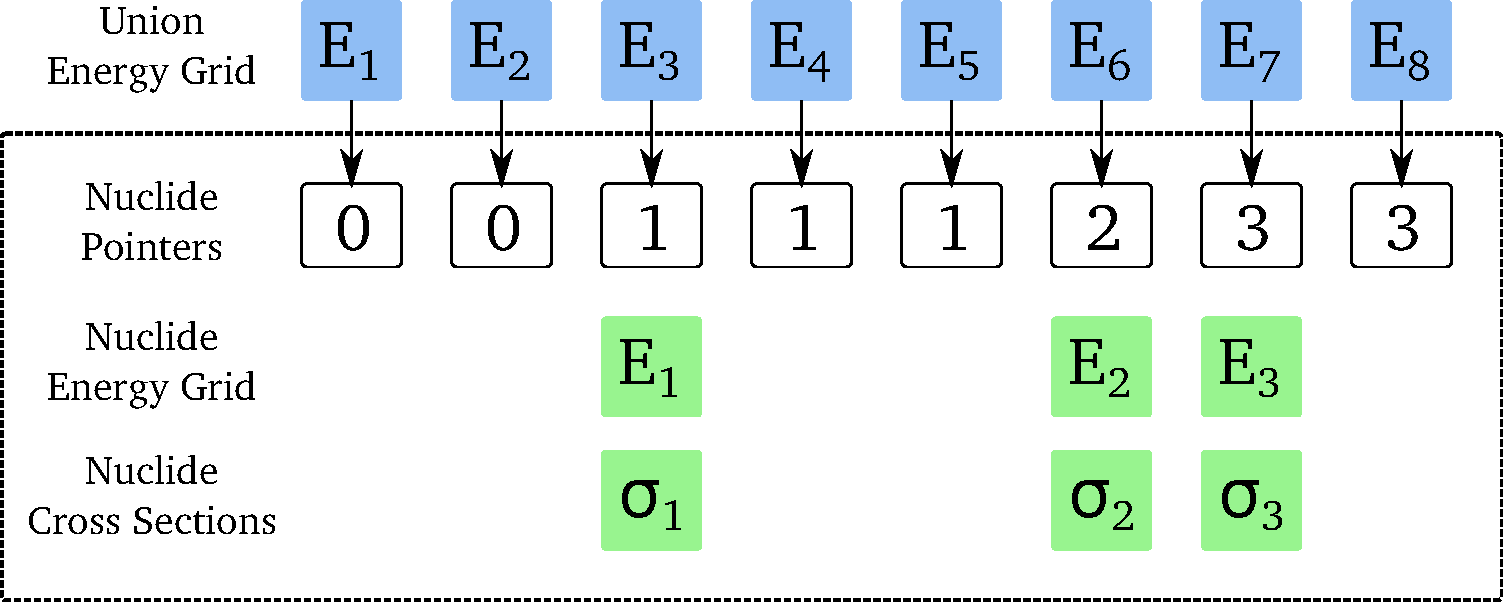
\includegraphics[width=6.0in]{figures/ch2/uniongrid.pdf}
  \caption{Mapping of union energy grid to nuclide energy grid through
    pointers.}
  \label{fig:uniongrid}
\end{figure}

\section{Random Number Generation}

In order to sample probability distributions, one must be able to produce random
numbers. The standard technique to do this is to generate numbers on the
interval $[0,1)$ from a deterministic sequence that has properties that make it
  appear to be random, e.g. being uniformly distributed and not exhibiting
  correlation between successive terms. Since the numbers produced this way are
  not truly ``random'' in a strict sense, they are typically referred to as
  pseudorandom numbers, and the techniques used to generate them are
  pseudorandom number generators (PRNGs). Numbers sampled on the unit interval
  can then be transformed for the purpose of sampling other continuous or
  discrete probability distributions.

There are a great number of algorithms for generating random numbers. One of the
simplest and commonly used algorithms is called a linear congruential generator
(LCG). We start with a random number \emph{seed} $\xi_0$ and a sequence of
random numbers can then be generated using the following recurrence relation:
\begin{equation}
  \label{eq:lcg}
  \xi_{i+1} = g \xi_i + c \mod M
\end{equation}
where $g$, $c$, and $M$ are constants. The choice of these constants will have a
profound effect on the quality and performance of the generator, so they should
not be chosen arbitrarily. As Donald Knuth stated in his seminal work \emph{The
  Art of Computer Programming} \cite{knuth-2006}, ``random numbers should not be
generated with a method chosen at random. Some theory should be used.''
Typically, $M$ is chosen to be a power of two as this enables $x \mod M$ to be
performed using the bitwise AND operator with a bit mask. The constants for the
linear congruential generator used by default in OpenMC are $g =
2806196910506780709$, $c = 1$, and $M = 2^{63}$ \cite{mathcomp-lecuyer-1999}.

One of the important capabilities for a random number generator is to be able to
skip ahead in the sequence of random numbers. Without this capability, it would
be very difficult to maintain reproducibility in a parallel calculation. If we
want to skip ahead $N$ random numbers and $N$ is large, the cost of sampling $N$
random numbers to get to that position may be prohibitively
expensive. Fortunately, algorithms have been developed that allow us to skip
ahead in $O(\log_2 N)$ operations instead of $O(N)$. One algorithm to do so is
described in a paper by Brown \cite{trans-brown-1994}. This algorithm relies on
the following relationship:
\begin{equation}
  \label{eq:lcg-skipahead}
  \xi_{i+k} = g^k \xi_i + c \frac{g^k - 1}{g - 1} \mod M
\end{equation}
Note that \eqref{eq:lcg-skipahead} has the same general form as \eqref{eq:lcg},
so the idea is to determine the new multiplicative and additive constants in
$O(\log_2 N)$ operations.

\section{Physics}

\subsection{Sampling Distance to Next Collision}

As a particle travels through a homogeneous material, the probability
distribution function for the distance to its next collision $\ell$ is
\begin{equation}
  \label{eq:distance-pdf}
  p(\ell) d\ell = \Sigma_t e^{-\Sigma_t \ell} d\ell
\end{equation}
where $\Sigma_t$ is the total macroscopic cross section of the
material. Equation \eqref{eq:distance-pdf} tells us that the further the
distance is to the next collision, the less likely the particle will travel that
distance. In order to sample the probability distribution function, we first
need to convert it to a cumulative distribution function
\begin{equation}
  \label{eq:distance-cdf}
  \int_0^{\ell} d\ell' p(\ell') = \int_0^{\ell} d\ell' \Sigma_t e^{-\Sigma_t
    \ell'} = 1 - e^{-\Sigma_t \ell}.
\end{equation}
By setting the cumulative distribution function equal to $\xi$, a random number
on the unit interval, and solving for the distance $\ell$, we obtain a formula
for sampling the distance to next collision:
\begin{equation}
  \label{eq:sample-distance-1}
  \ell = -\frac{\ln (1 - \xi)}{\Sigma_t}
\end{equation}
Since $\xi$ is uniformly distributed on $[0,1)$, this implies that $1 - \xi$ is
  also uniformly distributed on $[0,1)$ as well. Thus, the formula used to
    calculate the distance to next collision in OpenMC is
\begin{equation}
  \label{eq:sample-distance-2}
  \ell = -\frac{\ln \xi}{\Sigma_t}.
\end{equation}

\subsection{\texorpdfstring{$(n,\gamma)$}{(n,gamma)} and Other Disappearance Reactions}

All absorption reactions other than fission do not produce any secondary
neutrons. As a result, these are the easiest type of reactions to handle. When a
collision occurs, the first step is to sample a nuclide within a material. Once
the nuclide has been sampled, then a specific reaction for that nuclide is
sampled. Since the total absorption cross section is pre-calculated at the
beginning of a simulation, the first step in sampling a reaction is to determine
whether a ``disappearance'' reaction occurs where no secondary neutrons are
produced. This is done by sampling a random number $\xi$ on the interval $[0,1)$
  and checking whether
\begin{equation}
  \label{eq:disappearance}
  \xi \sigma_t (E) < \sigma_a (E) - \sigma_f (E)
\end{equation}
where $\sigma_t$ is the total cross section, $\sigma_a$ is the absorption cross
section (this includes fission), and $\sigma_f$ is the total fission cross
section. If this condition is met, then the neutron is killed and we proceed to
simulate the next neutron from the source bank.

No secondary particles from disappearance reactions such as photons or
alpha-particles are produced or tracked in OpenMC. To truly capture the affects
of gamma heating, it would be necessary to explicitly track photons originating
from $(n,\gamma)$ and other reactions.

\subsection{Elastic Scattering}

Elastic scattering refers to the process by which a neutron scatters off a
nucleus and does not leave it in an excited state. It is referred to as
``elastic'' because in the center-of-mass system, the neutron does not actually
lose energy. However, in lab coordinates, the neutron does indeed lose
energy. Elastic scattering can be treated exactly in a Monte Carlo code thanks
to its simplicity.

Let us discuss how OpenMC handles two-body elastic scattering kinematics. The
first step is to determine whether the target nucleus has any associated
motion. Above a certain energy threshold (400 kT by default), all scattering is
assumed to take place with the target at rest. Below this threshold though, we
must account for the thermal motion of the target nucleus. Methods to sample the
velocity of the target nucleus are described later in \autoref{sec:freegas}. For
the time being, let us assume that we have sampled the target velocity
$\mathbf{v}_t$. The velocity of the center-of-mass system is calculated as
\begin{equation}
  \label{eq:velocity-com}
  \mathbf{v}_{cm} = \frac{\mathbf{v}_n + A \mathbf{v}_t}{A + 1}
\end{equation}
where $\mathbf{v}_n$ is the velocity of the neutron and $A$ is the atomic mass
of the target nucleus measured in neutron masses (commonly referred to as the
\emph{atomic weight ratio}). With the velocity of the center-of-mass calculated,
we can then determine the neutron's velocity in the center-of-mass system:
\begin{equation}
  \label{eq:velocity-neutron-com}
  \mathbf{V}_n = \mathbf{v}_n - \mathbf{v}_{cm}
\end{equation}
where we have used uppercase $\mathbf{V}$ to denote the center-of-mass
system. The direction of the neutron in the center-of-mass system is
\begin{equation}
  \label{eq:angle-neutron-com}
  \mathbf{\Omega}_n = \frac{\mathbf{V}_n}{|| \mathbf{V}_n ||}.
\end{equation}
At low energies, elastic scattering will be isotropic in the center-of-mass
system, but for higher energies, there may be p-wave and higher order scattering
that leads to anisotropic scattering. Thus, in general, we need to sample a
cosine of the scattering angle which we will refer to as $\mu$. For elastic
scattering, the secondary angle distribution is always given in the
center-of-mass system and is sampled according to the procedure outlined in
\autoref{sec:sample-angle}. After the cosine of the angle of scattering has been
sampled, we need to determine the neutron's new direction $\mathbf{\Omega}'_n$
in the center-of-mass system. This is done with the procedure in
\autoref{sec:transform-coordinates}. The new direction is multiplied by the
speed of the neutron in the center-of-mass system to obtain the new velocity
vector in the center-of-mass:
\begin{equation}
  \label{eq:velocity-neutron-com-2}
  \mathbf{V}'_n = || \mathbf{V}_n || \mathbf{\Omega}'_n.
\end{equation}
Finally, we transform the velocity in the center-of-mass system back to lab
coordinates:
\begin{equation}
  \label{eq:velocity-neutron-lab}
  \mathbf{v}'_n = \mathbf{V}'_n + \mathbf{v}_{cm}.
\end{equation}
In OpenMC, the angle and energy of the neutron are stored rather than the
velocity vector itself, so the post-collision angle and energy can be inferred
from the post-collision velocity of the neutron in the lab system.

For tallies that require the scattering cosine, it is important to store the
scattering cosine in the lab system. If we know the scattering cosine in the
center-of-mass, the scattering cosine in the lab system can be calculated as
\begin{equation}
  \label{eq:cosine-lab}
  \mu_{lab} = \frac{1 + A\mu}{\sqrt{A^2 + 2A\mu + 1}}.
\end{equation}
However, \eqref{eq:cosine-lab} is only valid if the target was at rest. When the
target nucleus does have thermal motion, the cosine of the scattering angle can
be determined by simply taking the dot product of the neutron's initial and
final direction in the lab system.

\subsection{Inelastic Scattering}
\label{sec:inelastic-scatter}

The major algorithms for inelastic scattering were described in previous
sections. First, a scattering cosine is sampled using the algorithms in
\autoref{sec:sample-angle}. Then an outgoing energy is sampled using the
algorithms in \autoref{sec:sample-energy}. If the outgoing energy and scattering
cosine were given in the center-of-mass system, they are transformed to
laboratory coordinates using the algorithm described in
\autoref{sec:transform-coordinates}. Finally, the direction of the particle is
changed also using the procedure in \autoref{sec:transform-coordinates}.

Although inelastic scattering leaves the target nucleus in an excited state, no
secondary photons from nuclear de-excitation are tracked in OpenMC.

\subsection{$(n,xn)$ Reactions}

These types of reactions are just treated as inelastic scattering and as such
are subject to the same procedure as described in
\autoref{sec:inelastic-scatter}. Rather than tracking multiple secondary
neutrons, the weight of the outgoing neutron is multiplied by the number of
secondary neutrons, e.g. for $(n,2n)$, only one outgoing neutron is tracked but
its weight is doubled.

\subsection{Fission}
\label{sec:fission}

While fission is normally considered an absorption reaction, from the
perspective of a Monte Carlo simulation it actually bears more similarities to
inelastic scattering since fission results in secondary neutrons in the exit
channel. Other absorption reactions like $(n,\gamma)$ or $(n,\alpha)$, on the
contrary, produce no neutrons. There are a few other idiosyncrasies in treating
fission. In a criticality calculation, secondary neutrons from fission are only
``banked'' for use in the next generation rather than being tracked as secondary
neutrons from elastic and inelastic scattering would be. On top of this, fission
is sometimes broken into first-chance fission, second-chance fission, etc. An
ACE table either lists the partial fission reactions with secondary energy
distributions for each one, or a total fission reaction with a single secondary
energy distribution.

When a fission reaction is sampled in OpenMC (either total fission or, if data
exists, first- or second-chance fission), the following algorithm is used to
create and store fission sites for the following generation. First, the average
number of prompt and delayed neutrons must be determined to decide whether the
secondary neutrons will be prompt or delayed. This is important because delayed
neutrons have a markedly different spectrum from prompt neutrons, one that has a
lower average energy of emission. The total number of neutrons emitted $\nu_t$
is given as a function of incident energy in the ACE format. Two representations
exist for $\nu_t$. The first is a polynomial of order $N$ with coefficients
$c_0,c_1,\dots,c_N$. If $\nu_t$ has this format, we can evaluate it at incoming
energy $E$ by using the equation
\begin{equation}
  \label{eq:nu-polynomial}
  \nu_t (E) = \sum_{i = 0}^N c_i E^i.
\end{equation}
The other representation is just a tabulated function with a specified
interpolation law. The number of prompt neutrons released per fission event
$\nu_p$ is also given as a function of incident energy and can be specified in a
polynomial or tabular format. The number of delayed neutrons released per
fission event $\nu_d$ can only be specified in a tabular format. In practice, we
only need to determine $\nu_t$ and $\nu_d$. Once these have been determined, we
can calculate the delayed neutron fraction
\begin{equation}
  \label{eq:beta}
  \beta = \frac{\nu_d}{\nu_t}.
\end{equation}
We then need to determine how many total neutrons should be emitted from
fission. If survival biasing is not being used, then the number of neutrons
emitted is
\begin{equation}
  \label{eq:fission-neutrons}
  \nu = \frac{w \nu_t}{k_{eff}}
\end{equation}
where $w$ is the statistical weight and $k_{eff}$ is the effective
multiplication factor from the previous generation. The number of neutrons
produced is biased in this manner so that the expected number of fission
neutrons produced is the number of source particles that we started with in the
generation. Since $\nu$ is not an integer, we use the following procedure to
obtain an integral number of fission neutrons to produce. If $\xi > \nu -
\lfloor \nu \rfloor$, then we produce $\lfloor \nu \rfloor$ neutrons. Otherwise,
we produce $\lfloor \nu \rfloor + 1$ neutrons. Then, for each fission site
produced, we sample the outgoing angle and energy according to the algorithms
given in \autoref{sec:sample-angle} and \autoref{sec:sample-energy}
respectively. If the neutron is to be born delayed, then there is an extra step
of sampling a delayed neutron precursor group since they each have an associated
secondary energy distribution.

The sampled outgoing angle and energy of fission neutrons along with the
position of the collision site are stored in an array called the fission
bank. In a subsequent generation, these fission bank sites are used as starting
source sites.

\subsection{Sampling Secondary Angle Distributions}
\label{sec:sample-angle}

For any reactions with secondary neutrons, it is necessary to sample secondary
angle and energy distributions. This includes elastic and inelastic scattering,
fission, and $(n,xn)$ reactions. In some cases, the angle and energy
distributions may be specified separately, and in other cases, they may be
specified as a correlated angle-energy distribution. In the following sections,
we will outline the methods used to sample secondary distributions as well as
how they are used to modify the state of a particle.

For elastic scattering, it is only necessary to specify a secondary angle
distribution since the outgoing energy can be determined analytically. Other
reactions may also have separate secondary angle and secondary energy
distributions that are uncorrelated. In these cases, the secondary angle
distribution is represented as either
\begin{itemize}
\item An isotropic angular distribution,
\item An equiprobable distribution with 32 bins, or
\item A tabular distribution.
\end{itemize}

\subsubsection{Isotropic Angular Distribution}

In the first case, no data needs to be stored on the ACE table, and the cosine
of the scattering angle is simply calculated as
\begin{equation}
  \label{eq:isotropic-angle}
  \mu = 2\xi - 1
\end{equation}
where $\mu$ is the cosine of the scattering angle and $\xi$ is a random number
sampled uniformly on $[0,1)$.

\subsubsection{Equiprobable Angle Bin Distribution}

For a 32 equiprobable bin distribution, we select a random number $\xi$ to
sample a cosine bin $i$ such that
\begin{equation}
  \label{eq:equiprobable-bin}
  i = 1 + \lfloor 32\xi \rfloor.
\end{equation}
The same random number can then also be used to interpolate between neighboring
$\mu$ values to get the final scattering cosine:
\begin{equation}
  \label{eq:equiprobable-cosine}
  \mu = \mu_i + (32\xi - i) (\mu_{i+1} - \mu_i)
\end{equation}
where $\mu_i$ is the $i$th scattering cosine.

\subsubsection{Tabular Angular Distribution}
\label{sec:angle-tabular}

As the MCNP manual points out \cite{lanl-x5-2008}, using an equiprobable bin
distribution works well for high-probability regions of the scattering cosine,
but for low-probability regions it is not very accurate. Thus, a more accurate
method is to represent the scattering cosine with a tabular distribution. In
this case, we have a table of cosines and their corresponding values for a
probability distribution function and cumulative distribution function. For each
incoming neutron energy $E_i$, let us call $p_{i,j}$ the $j$th value in the
probability distribution function and $c_{i,j}$ the $j$th value in the
cumulative distribution function. We first find the interpolation factor on the
incoming energy grid:
\begin{equation}
  \label{eq:interpolation-factor}
  f = \frac{E - E_i}{E_{i+1} - E_i}
\end{equation}
where $E$ is the incoming energy of the particle. Then, statistical
interpolation is performed to choose between using the cosines and distribution
functions corresponding to energy $E_i$ and $E_{i+1}$. Let $\ell$ be the chosen
table where $\ell = i$ if $\xi_1 > f$ and $\ell = i + 1$ otherwise, and $\xi_1$
is a random number. Another random number $\xi_2$ is used to sample a scattering
cosine bin $j$ using the cumulative distribution function:
\begin{equation}
  \label{eq:sample-cdf}
  c_{\ell,j} < \xi_2 < c_{\ell,j+1}.
\end{equation}
The final scattering cosine will depend on whether histogram or linear-linear
interpolation is used. In general, we can write the cumulative distribution
function as
\begin{equation}
  \label{eq:cdf}
  c(\mu) = \int_{-1}^\mu p(\mu') d\mu'
\end{equation}
where $c(\mu)$ is the cumulative distribution function and $p(\mu)$
is the probability distribution function. Since we know that
$c(\mu_{\ell,j}) = c_{\ell,j}$, this implies that for $\mu >
\mu_{\ell,j}$,
\begin{equation}
  \label{eq:cdf-2}
  c(\mu) = c_{\ell,j} + \int_{\mu_{\ell,j}}^{\mu} p(\mu') d\mu'
\end{equation}

For histogram interpolation, we have that $p(\mu') = p_{\ell,j}$ for
$\mu_{\ell,j} \le \mu' < \mu_{\ell,j+1}$. Thus, after integrating
\eqref{eq:cdf-2} we have that
\begin{equation}
  \label{eq:cumulative-dist-histogram}
  c(\mu) = c_{\ell,j} + (\mu - \mu_{\ell,j}) p_{\ell,j} = \xi_2.
\end{equation}
Solving for the scattering cosine, we obtain the final form for histogram
interpolation:
\begin{equation}
  \label{eq:cosine-histogram}
  \mu = \mu_{\ell,j} + \frac{\xi_2 - c_{\ell,j}}{p_{\ell,j}}.
\end{equation}

For linear-linear interpolation, we represent the function $p(\mu')$ as a
first-order polynomial in $\mu'$. If we interpolate between successive values on
the probability distribution function, we have that
\begin{equation}
  \label{eq:pdf-interpolation}
    p(\mu') - p_{\ell,j} = \frac{p_{\ell,j+1} - p_{\ell,j}}{\mu_{\ell,j+1} -
    \mu_{\ell,j}} (\mu' - \mu_{\ell,j}).
\end{equation}
Solving for $p(\mu')$ in \eqref{eq:pdf-interpolation} and inserting it into
\eqref{eq:cdf-2}, we obtain
\begin{equation}
  \label{eq:cdf-linlin}
    c(\mu) = c_{\ell,j} + \int_{\mu_{\ell,j}}^{\mu} \left [ \frac{p_{\ell,j+1} -
    p_{\ell,j}}{\mu_{\ell,j+1} - \mu_{\ell,j}} (\mu' - \mu_{\ell,j}) +
    p_{\ell,j} \right ] d\mu'.
\end{equation}
Let us now make a change of variables using
\begin{equation}
  \label{eq:introduce-eta}
    \eta = \frac{p_{\ell,j+1} - p_{\ell,j}}{\mu_{\ell,j+1} - \mu_{\ell,j}}
    (\mu' - \mu_{\ell,j}) + p_{\ell,j}.
\end{equation}
Equation \eqref{eq:cdf-linlin} then becomes
\begin{equation}
  \label{eq:cdf-linlin-eta}
    c(\mu) = c_{\ell,j} + \frac{1}{m} \int_{p_{\ell,j}}^{m(\mu - \mu_{\ell,j}) +
    p_{\ell,j}} \eta \, d\eta
\end{equation}
where we have used
\begin{equation}
  \label{eq:slope}
    m = \frac{p_{\ell,j+1} - p_{\ell,j}}{\mu_{\ell,j+1} - \mu_{\ell,j}}.
\end{equation}
Integrating \eqref{eq:cdf-linlin-eta}, we have
\begin{equation}
  \label{eq:cdf-linlin-integrated}
    c(\mu) = c_{\ell,j} + \frac{1}{2m} \left ( \left [ m (\mu - \mu_{\ell,j} ) +
    p_{\ell,j} \right ]^2 - p_{\ell,j}^2 \right ) = \xi_2.
\end{equation}
Solving for $\mu$, we have the final form for the scattering cosine using a
tabular distribution and linear-linear interpolation:
\begin{equation}
  \label{eq:cosine-linlin}
    \mu = \mu_{\ell,j} + \frac{1}{m} \left ( \sqrt{p_{\ell,j}^2 + 2 m (\xi_2 -
    c_{\ell,j} )} - p_{\ell,j} \right ).
\end{equation}

\subsection{Sampling Secondary Energy and Correlated Angle/Energy Distributions}
\label{sec:sample-energy}

For a reaction with secondary neutrons, it is necessary to determine the
outgoing energy of the neutrons. For any reaction other than elastic scattering,
the outgoing energy must be determined based on tabulated or parameterized
data. The ENDF-6 Format \cite{bnl-herman-2009} specifies a variety of ways that
the secondary energy distribution can be represented. ENDF File 5 contains
uncorrelated energy distribution whereas ENDF File 6 contains correlated
energy-angle distributions. The ACE format specifies its own representations
based loosely on the formats given in ENDF-6. In this section, we will describe
how the outgoing energy of secondary particles is determined based on each ACE
law.

One of the subtleties in the ACE format is the fact that a single reaction can
have multiple secondary energy distributions. This is mainly useful for
reactions with multiple neutrons in the exit channel such as $(n,2n)$ or
$(n,3n)$. In these types of reactions, each neutron is emitted corresponding to
a different excitation level of the compound nucleus, and thus in general the
neutrons will originate from different energy distributions. If multiple energy
distributions are present, they are assigned probabilities that can then be used
to randomly select one.

Once a secondary energy distribution has been sampled, the procedure for
determining the outgoing energy will depend on which ACE law has been specified
for the data.

\subsubsection{ACE Law 1 - Tabular Equiprobable Energy Bins}
\label{sec:ace-law-1}

In the tabular equiprobable bin representation, an array of equiprobable
outgoing energy bins is given for a number of incident energies. While the
representation itself is simple, the complexity lies in how one interpolates
between incident as well as outgoing energies on such a table. If one performs
simple interpolation between tables for neighboring incident energies, it is
possible that the resulting energies would violate laws governing the
kinematics, i.e. the outgoing energy may be outside the range of available
energy in the reaction.

To avoid this situation, the accepted practice is to use a process known as
scaled interpolation \cite{nse-doyas-1972}. First, we find the tabulated
incident energies which bound the actual incoming energy of the particle,
i.e. find $i$ such that $E_i < E < E_{i+1}$ and calculate the interpolation
factor $f$ via \eqref{eq:interpolation-factor}. Then, we interpolate between the
minimum and maximum energies of the outgoing energy distributions corresponding
to $E_i$ and $E_{i+1}$:
\begin{equation}
  \label{eq:ace-law-1-minmax}
  \begin{split}
    E_{min} &= E_{i,1} + f ( E_{i+1,1} - E_i ) \\
    E_{max} &= E_{i,M} + f ( E_{i+1,M} - E_M )
  \end{split}
\end{equation}
where $E_{min}$ and $E_{max}$ are the minimum and maximum outgoing energies of a
scaled distribution, $E_{i,j}$ is the $j$th outgoing energy corresponding to the
incoming energy $E_i$, and $M$ is the number of outgoing energy bins. Next,
statistical interpolation is performed to choose between using the outgoing
energy distributions corresponding to energy $E_i$ and $E_{i+1}$. Let $\ell$ be
the chosen table where $\ell = i$ if $\xi_1 > f$ and $\ell = i + 1$ otherwise,
and $\xi_1$ is a random number. Now, we randomly sample an equiprobable outgoing
energy bin $j$ and interpolate between successive values on the outgoing energy
distribution:
\begin{equation}
  \label{eq:ace-law-1-intermediate}
  \hat{E} = E_{\ell,j} + \xi_2 (E_{\ell,j+1} - E_{\ell,j})
\end{equation}
where $\xi_2$ is a random number sampled uniformly on $[0,1)$. Since
this outgoing energy may violate reaction kinematics, we then scale it to the
minimum and maximum energies we calculated earlier to get the final outgoing
energy:
\begin{equation}
  \label{eq:ace-law-1-energy}
  E' = E_{min} + \frac{\hat{E} - E_{\ell,1}}{E_{\ell,M} - E_{\ell,1}}
  (E_{max} - E_{min}).
\end{equation}

\subsubsection{ACE Law 3 - Inelastic Level Scattering}

It can be shown \cite{foderaro-1971} that in inelastic level scattering, the
outgoing energy of the neutron $E'$ can be related to the Q-value of the
reaction and the incoming energy:
\begin{equation}
  \label{eq:level-scattering}
  E' = \left ( \frac{A}{A+1} \right )^2 \left ( E - \frac{A + 1}{A} Q \right )
\end{equation}
where $A$ is the mass of the target nucleus measured in neutron masses.

\subsubsection{ACE Law 4 - Continuous Tabular Distribution}
\label{sec:ace-law-4}

This representation is very similar that in \autoref{sec:ace-law-1} except that
instead of equiprobable outgoing energy bins, the outgoing energy distribution
for each incoming energy is represented with a probability distribution
function. For each incoming neutron energy $E_i$, let us call $p_{i,j}$ the
$j$th value in the probability distribution function, $c_{i,j}$ the $j$th value
in the cumulative distribution function, and $E_{i,j}$ the $j$th outgoing
energy.

We proceed first as we did for ACE Law 1, determining the bounding energies of
the particle's incoming energy such that $E_i < E < E_{i+1}$ and calculating an
interpolation factor $f$ with \eqref{eq:interpolation-factor}. Next, statistical
interpolation is performed to choose between using the outgoing energy
distributions corresponding to energy $E_i$ and $E_{i+1}$. Let $\ell$ be the
chosen table where $\ell = i$ if $\xi_1 > f$ and $\ell = i + 1$ otherwise, and
$\xi_1$ is a random number. Then, we sample an outgoing energy bin $j$ using the
cumulative distribution function:
\begin{equation}
  \label{eq:ace-law-4-sample-cdf}
  c_{\ell,j} < \xi_2 < c_{\ell,j+1}
\end{equation}
where $\xi_2$ is a random number sampled uniformly on $[0,1)$. At this point, we
  need to interpolate between the successive values on the outgoing energy
  distribution using either histogram or linear-linear interpolation. The
  formulas for these can be derived along the same lines as those found in
  \autoref{sec:angle-tabular}. For histogram interpolation, the interpolated
  outgoing energy on the $\ell$th distribution is
\begin{equation}
  \label{eq:energy-histogram}
  \hat{E} = E_{\ell,j} + \frac{\xi_2 - c_{\ell,j}}{p_{\ell,j}}
\end{equation}
If linear-linear interpolation is to be used, the outgoing energy on the
$\ell$th distribution is
\begin{equation}
  \label{eq:energy-linlin}
  \hat{E} = E_{\ell,j} + \frac{E_{\ell,j+1} - E_{\ell,j}}{p_{\ell,j+1} -
    p_{\ell,j}} \left ( \sqrt{p_{\ell,j}^2 + 2 \frac{p_{\ell,j+1} -
      p_{\ell,j}}{E_{\ell,j+1} - E_{\ell,j}} ( \xi_2 - c_{\ell,j} )} -
  p_{\ell,j} \right )
\end{equation}
Since this outgoing energy may violate reaction kinematics, we then scale it to
minimum and maximum energies interpolated between the neighboring outgoing
energy distributions to get the final outgoing energy:
\begin{equation}
  \label{eq:ace-law-4-energy}
  E' = E_{min} + \frac{\hat{E} - E_{\ell,1}}{E_{\ell,M} - E_{\ell,1}}
  (E_{max} - E_{min})
\end{equation}
where $E_{min}$ and $E_{max}$ are defined the same as in
\eqref{eq:ace-law-1-minmax}.

\subsubsection{ACE Law 7 - Maxwell Fission Spectrum}
\label{sec:maxwell}

One representation of the secondary energies for neutrons from fission is the
so-called Maxwell spectrum. A probability distribution for the Maxwell spectrum
can be written in the form
\begin{equation}
  \label{eq:maxwell-spectrum}
  p(E') dE' = c E'^{1/2} e^{-E'/T(E)} dE'
\end{equation}
where $E$ is the incoming energy of the neutron and $T$ is the so-called nuclear
temperature, which is a function of the incoming energy of the neutron. The ACE
format contains a list of nuclear temperatures versus incoming energies. The
nuclear temperature is interpolated between neighboring incoming energies using
a specified interpolation law. Once the temperature $T$ is determined, we then
calculate a candidate outgoing energy based on rule C64 in the Monte Carlo
Sampler \cite{lanl-everett-1983}:
\begin{equation}
  \label{eq:maxwell-E-candidate}
  E' = -T \left [ \log (\xi_1) + \log (\xi_2) \cos^2 \left ( \frac{\pi
      \xi_3}{2} \right ) \right ]
\end{equation}
where $\xi_1, \xi_2, \xi_3$ are random numbers sampled on the unit
interval. The outgoing energy is only accepted if
\begin{equation}
  \label{eq:maxwell-restriction}
  0 \le E' \le E - U
\end{equation}
where $U$ is called the restriction energy and is specified on the ACE table. If
the outgoing energy is rejected, it is resampled using
\eqref{eq:maxwell-E-candidate}.

\subsubsection{ACE Law 9 - Evaporation Spectrum}

Evaporation spectra are primarily used in compound nucleus processes where a
secondary particle can ``evaporate'' from the compound nucleus if it has
sufficient energy. The probability distribution for an evaporation spectrum can
be written in the form
\begin{equation}
  \label{eq:evaporation-spectrum}
  p(E') dE' = c E' e^{-E'/T(E)} dE'
\end{equation}
where $E$ is the incoming energy of the neutron and $T$ is the nuclear
temperature, which is a function of the incoming energy of the neutron. The ACE
format contains a list of nuclear temperatures versus incoming energies. The
nuclear temperature is interpolated between neighboring incoming energies using
a specified interpolation law. Once the temperature $T$ is determined, we then
calculate a candidate outgoing energy based on rule C45 in the Monte Carlo
Sampler \cite{lanl-everett-1983}:
\begin{equation}
  \label{eq:evaporation-E}
  E' = -T \log (\xi_1 \xi_2)
\end{equation}
where $\xi_1, \xi_2$ are random numbers sampled on the unit interval. The
outgoing energy is only accepted according to a specified restriction energy as
in \eqref{eq:maxwell-restriction}.

\subsubsection{ACE Law 11 - Energy-Dependent Watt Spectrum}

The probability distribution for a Watt fission spectrum
\cite{physrev-watt-1952} can be written in the form
\begin{equation}
  \label{eq:watt-spectrum}
  p(E') dE' = c e^{-E'/a(E)} \sinh \sqrt{b(E) \, E'} dE'
\end{equation}
where $a$ and $b$ are parameters for the distribution and are given as tabulated
functions of the incoming energy of the neutron. These two parameters are
interpolated on the incoming energy grid using a specified interpolation
law. Once the parameters have been determined, we sample a Maxwellian spectrum
with nuclear temperature $a$ using the algorithm described in
\autoref{sec:maxwell} to get an energy $W$. Then, the outgoing energy is
calculated as
\begin{equation}
  \label{eq:watt-E}
  E' = W + \frac{a^2 b}{4} + (2\xi - 1) \sqrt{a^2 b W}
\end{equation}
where $\xi$ is a random number sampled on the interval $[0,1)$. The outgoing
  energy is only accepted according to a specified restriction energy $U$ as
  defined in \eqref{eq:maxwell-restriction}.

This algorithm can be found in Forrest Brown's lectures on Monte Carlo methods
\cite{lanl-brown-2005} and is an unpublished sampling scheme based on the
original Watt spectrum derivation.

\subsubsection{ACE Law 44 - Kalbach-Mann Correlated Scattering}

This law is very similar to ACE Law 4 except now the outgoing angle of the
neutron is correlated to the outgoing energy and is not sampled from a separate
distribution. For each incident neutron energy $E_i$ tabulated, there is
an array of precompound factors $R_{i,j}$ and angular distribution slopes
$A_{i,j}$ corresponding to each outgoing energy bin $j$ in addition
to the outgoing energies and distribution functions as in ACE Law 4.

The calculation of the outgoing energy of the neutron proceeds exactly the same
as in the algorithm described in \autoref{sec:ace-law-4}. In that algorithm, we
found an interpolation factor $f$, statistically sampled an incoming energy bin
$\ell$, and sampled an outgoing energy bin $j$ based on the tabulated cumulative
distribution function. Once the outgoing energy has been determined with
\eqref{eq:ace-law-4-energy}, we then need to calculate the outgoing angle based
on the tabulated Kalbach-Mann parameters. These parameters themselves are
subject to either histogram or linear-linear interpolation on the outgoing
energy grid. For histogram interpolation, the parameters are
\begin{equation}
  \label{eq:KM-parameters-histogram}
  \begin{split}
    R &= R_{\ell,j} \\ 
    A &= A_{\ell,j}
  \end{split}
\end{equation}
If linear-linear interpolation is specified, the parameters are
\begin{equation}
  \label{eq:KM-parameters-linlin}
  \begin{split}
    R &= R_{\ell,j} + \frac{\hat{E} - E_{\ell,j}}{E_{\ell,j+1} - E_{\ell,j}} (
    R_{\ell,j+1} - R_{\ell,j} ) \\
    A &= A_{\ell,j} + \frac{\hat{E} - E_{\ell,j}}{E_{\ell,j+1} - E_{\ell,j}} (
    A_{\ell,j+1} - A_{\ell,j} )
  \end{split}
\end{equation}
where $\hat{E}$ is defined in \eqref{eq:energy-linlin}. With the parameters
determined, the probability distribution function for the cosine of the
scattering angle is
\begin{equation}
  \label{eq:KM-pdf-angle}
  p(\mu) d\mu = \frac{A}{2 \sinh (A)} \left [ \cosh (A\mu) + R \sinh (A\mu)
    \right ] d\mu
\end{equation}
The rules for sampling this probability distribution function can be derived
based on rules C39 and C40 in the Monte Carlo Sampler
\cite{lanl-everett-1983}. First, we sample two random numbers $\xi_3, \xi_4$ on
the unit interval. If $\xi_3 > R$ then the outgoing angle is
\begin{equation}
  \label{eq:KM-angle-1}
  \mu = \frac{1}{A} \ln \left ( T + \sqrt{T^2 + 1} \right )
\end{equation}
where $T = (2 \xi_4 - 1) \sinh (A)$. If $\xi_3 \le R$, then the
outgoing angle is
\begin{equation}
  \label{eq:KM-angle-2}
  \mu = \frac{1}{A} \ln \left ( \xi_4 e^A + (1 - \xi_4) e^{-A} \right )
\end{equation}

\subsubsection{ACE Law 61 - Correlated Energy and Angle Distribution}

This law is very similar to ACE Law 44 in the sense that the outgoing angle of
the neutron is correlated to the outgoing energy and is not sampled from a
separate distribution. In this case though, rather than being determined from an
analytical distribution function, the cosine of the scattering angle is
determined from a tabulated distribution. For each incident energy $i$ and
outgoing energy $j$, there is a tabulated angular distribution.

The calculation of the outgoing energy of the neutron proceeds exactly the same
as in the algorithm described in \autoref{sec:ace-law-4}. In that algorithm, we
found an interpolation factor $f$, statistically sampled an incoming energy bin
$\ell$, and sampled an outgoing energy bin $j$ based on the tabulated cumulative
distribution function. Once the outgoing energy has been determined with
\eqref{eq:ace-law-4-energy}, we then need to decide which angular distribution
to use. If histogram interpolation was used on the outgoing energy bins, then we
use the angular distribution corresponding to incoming energy bin $\ell$ and
outgoing energy bin $j$. If linear-linear interpolation was used on the outgoing
energy bins, then we use whichever angular distribution was closer to the
sampled value of the cumulative distribution function for the outgoing
energy. The actual algorithm used to sample the chosen tabular angular
distribution has been previously described in \autoref{sec:angle-tabular}.

\subsubsection{ACE Law 66 - N-Body Phase Space Distribution}

Reactions in which there are more than two products of similar masses are
sometimes best treated by using what's known as an N-body phase
distribution. This distribution has the following probability density function
for outgoing energy of the $i$th particle in the center-of-mass system:
\begin{equation}
  \label{eq:n-body-pdf}
  p_i(E') dE' = C_n \sqrt{E'} (E_i^{max} - E')^{(3n/2) - 4} dE'
\end{equation}
where $n$ is the number of outgoing particles, $C_n$ is a normalization
constant, $E_i^{max}$ is the maximum center-of-mass energy for particle $i$, and
$E'$ is the outgoing energy. The algorithm for sampling the outgoing energy is
based on algorithms R28, C45, and C64 in the Monte Carlo Sampler
\cite{lanl-everett-1983}. First we calculate the maximum energy in the
center-of-mass using the following equation:
\begin{equation}
  \label{eq:n-body-emax}
  E_i^{max} = \frac{A_p - 1}{A_p} \left ( \frac{A}{A+1} E + Q \right )
\end{equation}
where $A_p$ is the total mass of the outgoing particles in neutron masses, $A$
is the mass of the original target nucleus in neutron masses, and $Q$ is the
Q-value of the reaction. Next we sample a value $x$ from a Maxwell distribution
with a nuclear temperature of one using the algorithm outlined in
\autoref{sec:maxwell}. We then need to determine a value $y$ that will depend on
how many outgoing particles there are. For $n = 3$, we simply sample another
Maxwell distribution with unity nuclear temperature. For $n = 4$, we use the
equation
\begin{equation}
  \label{eq:n-body-y4}
  y = -\ln ( \xi_1 \xi_2 \xi_3 )
\end{equation}
where $\xi_i$ are random numbers sampled on the interval
$[0,1)$. For $n = 5$, we use the equation
\begin{equation}
  \label{eq:n-body-y5}
  y = -\ln ( \xi_1 \xi_2 \xi_3 \xi_4 ) - \ln ( \xi_5 ) \cos^2 \left (
  \frac{\pi}{2} \xi_6 \right )
\end{equation}
After $x$ and $y$ have been determined, the outgoing energy is then
calculated as
\begin{equation}
  \label{eq:n-body-energy}
  E' = \frac{x}{x + y} E_i^{max}
\end{equation}
There are two important notes to make regarding the N-body phase space
distribution. First, the documentation (and code) for MCNP5-1.60 has a mistake
in the algorithm for $n = 4$. That being said, there are no existing nuclear
data evaluations which use an N-body phase space distribution with $n = 4$, so
the error would not affect any calculations. In the ENDF/B-VII.0 nuclear data
evaluation, only one reaction uses an N-body phase space distribution at all,
the $(n,2n)$ reaction with $^2$H.

\subsection{Transforming a Particle's Coordinates}
\label{sec:transform-coordinates}

Once the cosine of the scattering angle $\mu$ has been sampled either from an
angle distribution or a correlated angle-energy distribution, we are still left
with the task of transforming the particle's coordinates. If the outgoing energy
and scattering cosine were given in the center-of-mass system, then we first
need to transform these into the laboratory system. The relationship between the
outgoing energy in center-of-mass and laboratory is
\begin{equation}
  \label{eq:energy-com-to-lab}
  E' = E'_{cm} + \frac{E + 2\mu_{cm} (A + 1) \sqrt{EE'_{cm}}}{(A+1)^2}
\end{equation}
where $E'_{cm}$ is the outgoing energy in the center-of-mass system,
$\mu_{cm}$ is the scattering cosine in the center-of-mass system,
$E'$ is the outgoing energy in the laboratory system, and $E$ is the
incident neutron energy. The relationship between the scattering cosine in
center-of-mass and laboratory is
\begin{equation}
  \label{eq:angle-com-to-lab}
  \mu = \mu_{cm} \sqrt{\frac{E'_{cm}}{E'}} + \frac{1}{A + 1}
  \sqrt{\frac{E}{E'}}
\end{equation}
where $\mu$ is the scattering cosine in the laboratory system. The
scattering cosine still only tells us the cosine of the angle between the
original direction of the particle and the new direction of the particle. If we
express the pre-collision direction of the particle as $\mathbf{\Omega} =
(u,v,w)$ and the post-collision direction of the particle as
$\mathbf{\Omega}' = (u',v',w')$, it is possible to relate the pre- and
post-collision components. We first need to uniformly sample an azimuthal angle
$\phi$ in $[0, 2\pi)$. After the azimuthal angle has been sampled,
the post-collision direction is calculated as
\begin{equation}
  \label{eq:post-collision-angle}
  \begin{split}
    u' &= \mu u + \frac{\sqrt{1 - \mu^2} ( uw \cos\phi - v \sin\phi )}{\sqrt{1 -
        w^2}} \\
    v' &= \mu v + \frac{\sqrt{1 - \mu^2} ( vw \cos\phi + u \sin\phi )}{\sqrt{1 -
        w^2}} \\
    w' &= \mu w - \sqrt{1 - \mu^2} \sqrt{1 - w^2} \cos\phi.
  \end{split}
\end{equation}

\subsection{Effect of Thermal Motion on Cross Sections}
\label{sec:freegas}

When a neutron scatters off of a nucleus, it may often be assumed that the
target nucleus is at rest. However, the target nucleus will have motion
associated with its thermal vibration, even at absolute zero\footnote{This is
  due to the zero-point energy arising from quantum mechanical
  considerations.}. Thus, the velocity of the neutron relative to the target
nucleus is in general not the same as the velocity of the neutron entering the
collision.

The effect of the thermal motion on the interaction probability can be written
as
\begin{equation}
  \label{eq:doppler-broaden}
  v_n \bar{\sigma} (v_n, T) = \int d\mathbf{v}_T v_r \sigma(v_r)
  M (\mathbf{v}_T)
\end{equation}
where $v_n$ is the magnitude of the velocity of the neutron, $\bar{\sigma}$ is
an effective cross section, $T$ is the temperature of the target material,
$\mathbf{v}_T$ is the velocity of the target nucleus, $v_r = || \mathbf{v}_n -
\mathbf{v}_T ||$ is the magnitude of the relative velocity, $\sigma$ is the
cross section at 0 K, and $M (\mathbf{v}_T)$ is the probability distribution for
the target nucleus velocity at temperature $T$ (a Maxwellian). In a Monte Carlo
code, one must account for the effect of the thermal motion on both the
integrated cross section as well as secondary angle and energy
distributions. For integrated cross sections, it is possible to calculate
thermally-averaged cross sections by applying a kernel Doppler broadening
algorithm to data at 0 K (or some temperature lower than the desired
temperature). The most ubiquitous algorithm for this purpose is the SIGMA1
method \cite{nse-cullen-1976} developed by Red Cullen and subsequently refined
by others. This method is used in the NJOY \cite{nds-macfarlane-2010} and PREPRO
\cite{iaea-cullen-2012} data processing codes.

The effect of thermal motion on secondary angle and energy distributions can be
accounted for on-the-fly in a Monte Carlo simulation. We must first qualify
where it is actually used however. All threshold reactions are treated as being
independent of temperature, and therefore they are not Doppler broadened in NJOY
and no special procedure is used to adjust the secondary angle and energy
distributions. The only non-threshold reactions with secondary neutrons are
elastic scattering and fission. For fission, it is assumed that the neutrons are
emitted isotropically (this is not strictly true, but is nevertheless a good
approximation). This leaves only elastic scattering that needs a special thermal
treatment for secondary distributions.

Fortunately, it is possible to directly sample the velocity of the target
nuclide and use it in the kinematic calculations. However, this calculation is a
bit more nuanced than it might seem at first glance. One might be tempted to
simply sample a Maxwellian distribution for the velocity of the target nuclide.
Careful inspection of \eqref{eq:doppler-broaden} however tells us that target
velocities that produce relative velocities which correspond to high cross
sections will have a greater contribution to the effective reaction rate. This
is most important when the velocity of the incoming neutron is close to a
resonance. For example, if the neutron's velocity corresponds to a local minimum
in a resonance elastic scattering cross section, a very small target velocity
can cause the relative velocity to correspond to the peak of the resonance, thus
making a disproportionate contribution to the reaction rate. The conclusion is
that if we are to sample a target velocity in the Monte Carlo code, it must be
done in such a way that preserves the thermally-averaged reaction rate as per
\eqref{eq:doppler-broaden}.

The method by which most Monte Carlo codes sample the target velocity for use in
elastic scattering kinematics is outlined in detail by Gelbard
\cite{anl-gelbard-1979}. The derivation here largely follows that of
Gelbard. Let us first write the reaction rate as a function of the velocity of
the target nucleus:
\begin{equation}
  \label{eq:reaction-rate}
  R(\mathbf{v}_T) = || \mathbf{v}_n - \mathbf{v}_T || \sigma ( ||
  \mathbf{v}_n - \mathbf{v}_T || ) M ( \mathbf{v}_T )
\end{equation}
where $R$ is the reaction rate. Note that this is just the right-hand side of
\eqref{eq:doppler-broaden}. Based on the discussion above, we want to construct
a probability distribution function for sampling the target velocity to preserve
the reaction rate --- this is different from the overall probability
distribution function for the target velocity, $M ( \mathbf{v}_T )$. This
probability distribution function can be found by integrating
\eqref{eq:reaction-rate} to obtain a normalization factor:
\begin{equation}
  \label{eq:target-pdf-1}
  p( \mathbf{v}_T ) d\mathbf{v}_T = \frac{R(\mathbf{v}_T) d\mathbf{v}_T}{\int
    d\mathbf{v}_T \, R(\mathbf{v}_T)}
\end{equation}
Let us call the normalization factor in the denominator of
\eqref{eq:target-pdf-1} $C$.

It is normally assumed that $\sigma (v_r)$ is constant over the range of
relative velocities of interest. This is a good assumption for almost all cases
since the elastic scattering cross section varies slowly with velocity for light
nuclei, and for heavy nuclei where large variations can occur due to resonance
scattering, the moderating effect is rather small. Nonetheless, this assumption
may cause incorrect answers in systems with low-lying resonances that can cause
a significant amount of up-scatter that would be ignored by this assumption
(e.g. $^{238}U$ in commercial light-water reactors). Nevertheless, with this
assumption, we write $\sigma (v_r) = \sigma_s$ which simplifies
\eqref{eq:target-pdf-1} to
\begin{equation}
  \label{eq:target-pdf-2}
  p( \mathbf{v}_T ) d\mathbf{v}_T = \frac{\sigma_s}{C} || \mathbf{v}_n -
  \mathbf{v}_T || M ( \mathbf{v}_T ) d\mathbf{v}_T.
\end{equation}
The Maxwellian distribution in velocity is
\begin{equation}
  \label{eq:maxwellian-velocity}
  M (\mathbf{v}_T) = \left ( \frac{m}{2\pi kT} \right )^{3/2} \exp \left (
  \frac{-m || \mathbf{v}_T ||^2}{2kT} \right )
\end{equation}
where $m$ is the mass of the target nucleus and $k$ is Boltzmann's
constant. Notice here that the term in the exponential is dependent only on the
speed of the target, not on the actual direction. Thus, we can change the
Maxwellian into a distribution for speed rather than velocity. The differential
element of velocity is
\begin{equation}
  \label{eq:differential-velocity}
  d\mathbf{v}_T = v_T^2 dv_T d\mu d\phi.
\end{equation}
Let us define the Maxwellian distribution in speed as
\begin{equation}
  \label{eq:maxwellian-speed}
  M (v_T) dv_T = \int_{-1}^1 d\mu \int_{0}^{2\pi} d\phi \, dv_T \, v_T^2
  M(\mathbf{v}_T) = \sqrt{ \frac{2}{\pi} \left ( \frac{m}{kT} \right )^3}
  v_T^2 \exp \left ( \frac{-m v_T}{2kT} \right ) dv_T.
\end{equation}
To simplify things a bit, we'll define a parameter
\begin{equation}
  \label{eq:maxwellian-beta}
  \beta = \sqrt{\frac{m}{2kT}}.
\end{equation}
Substituting \eqref{eq:maxwellian-beta} into \eqref{eq:maxwellian-speed}, we
obtain
\begin{equation}
  \label{eq:maxwellian-speed2}
  M (v_T) dv_T = \frac{4}{\sqrt{\pi}} \beta^3 v_T^2 \exp \left ( -\beta^2
  v_T^2 \right ) dv_T.
\end{equation}
Now, changing variables in \eqref{eq:target-pdf-2} by using the result from
\eqref{eq:maxwellian-speed2}, our new probability distribution function is
\begin{equation}
  \label{eq:target-pdf-3}
  p( v_T, \mu ) dv_T d\mu = \frac{4\sigma_s}{\sqrt{\pi}C'} || \mathbf{v}_n -
  \mathbf{v}_T || \beta^3 v_T^2 \exp \left ( -\beta^2 v_T^2 \right ) dv_T d\mu.
\end{equation}
Again, the Maxwellian distribution for the speed of the target nucleus has no
dependence on the angle between the neutron and target velocity vectors. Thus,
only the term $|| \mathbf{v}_n - \mathbf{v}_T ||$ imposes any constraint
on the allowed angle. Our last task is to take that term and write it in terms
of magnitudes of the velocity vectors and the angle rather than the vectors
themselves. We can establish this relation based on the law of cosines which
tells us that
\begin{equation}
  \label{eq:lawcosine}
  2 v_n v_T \mu = v_n^2 + v_T^2 - v_r^2.
\end{equation}
Thus, we can infer that
\begin{equation}
  \label{eq:change-terms}
  || \mathbf{v}_n - \mathbf{v}_T || = || \mathbf{v}_r || = v_r = \sqrt{v_n^2 +
    v_T^2 - 2v_n v_T \mu}
\end{equation}
Inserting \eqref{eq:change-terms} into \eqref{eq:target-pdf-3}, we obtain
\begin{equation}
  \label{eq:target-pdf-4}
  p( v_T, \mu ) dv_T d\mu = \frac{4\sigma_s}{\sqrt{\pi}C'} \sqrt{v_n^2 +
    v_T^2 - 2v_n v_T \mu} \beta^3 v_T^2 \exp \left ( -\beta^2 v_T^2 \right )
  dv_T d\mu
\end{equation}
This expression is still quite formidable and does not lend itself to any
natural sampling scheme. We can divide this probability distribution into two
parts as such:
\begin{align}
  \label{eq:divide-pdf-p}
  p(v_T, \mu) &= f_1(v_T, \mu) f_2(v_T) \\
  \label{eq:divide-pdf-f1}
  f_1(v_T, \mu) &= \frac{4\sigma_s}{\sqrt{\pi} C'} \frac{ \sqrt{v_n^2 + v_T^2 -
      2v_n v_T \mu}}{v_n + v_T} \\
  \label{eq:divide-pdf-f2}
  f_2(v_T) &= (v_n + v_T) \beta^3 v_T^2 \exp \left ( -\beta^2 v_T^2 \right )
\end{align}
In general, any probability distribution function of the form $p(x) =
f_1(x) f_2(x)$ with $f_1(x)$ bounded can be sampled by sampling
$x'$ from the distribution
\begin{equation}
  \label{eq:freegas-f2}
  q(x) dx = \frac{f_2(x) dx}{\int f_2(x) dx}
\end{equation}
and accepting it with probability
\begin{equation}
  \label{eq:freegas-accept}
  p_{accept} = \frac{f_1(x')}{\max f_1(x)}
\end{equation}
The reason for dividing and multiplying the terms by $v_n + v_T$ is to ensure
that the first term is bounded. In general, $|| \mathbf{v}_n - \mathbf{v}_T ||$
can take on arbitrarily large values, but if we divide it by its maximum value
$v_n + v_T$, then it ensures that the function will be bounded. We now must come
up with a sampling scheme for \eqref{eq:freegas-f2}. To determine $q(v_T)$, we
need to integrate $f_2$ in \eqref{eq:divide-pdf-f2}. Doing so we find that
\begin{equation}
  \label{eq:integrate-f2}
  \int_0^{\infty} dv_T (v_n + v_T) \beta^3 v_T^2 \exp \left ( -\beta^2 v_T^2
  \right ) = \frac{1}{4\beta} \left ( \sqrt{\pi} \beta v_n + 2 \right ).
\end{equation}
Thus, we need to sample the probability distribution function
\begin{equation}
  \label{eq:freegas-f2-2}
  q(v_T) dv_T = \left ( \frac{4\beta^2 v_n v_T^2}{\sqrt{\pi} \beta v_n + 2} +
  \frac{4\beta^4 v_T^3}{\sqrt{\pi} \beta v_n + 2} \right ) exp \left (
  -\beta^2 v_T^2 \right )
\end{equation}
Now, let us do a change of variables with the following definitions
\begin{equation}
  \label{eq:beta-to-x}
  \begin{split}
    x &= \beta v_T \\
    y &= \beta v_n.
  \end{split}
\end{equation}
Substituting \eqref{eq:beta-to-x} into \eqref{eq:freegas-f2-2} along with $dx =
\beta dv_T$ and doing some crafty rearranging of terms yields
\begin{equation}
  \label{eq:freegas-f2-3}
  q(x) dx = \left [ \left ( \frac{\sqrt{\pi} y}{\sqrt{\pi} y + 2} \right )
    \frac{4}{\sqrt{\pi}} x^2 e^{-x^2} + \left ( \frac{2}{\sqrt{\pi} y + 2}
    \right ) 2x^3 e^{-x^2} \right ] dx.
\end{equation}
It's important to note the following two facts. First, the terms outside the
parentheses are properly normalized probability distribution functions that can
be sampled directly. Secondly, the terms inside the parentheses are always less
than unity. Thus, the sampling scheme for $q(x)$ is as follows. We sample a
random number $\xi_1$ on the interval $[0,1)$ and if
\begin{equation}
  \label{eq:freegas-alpha}
  \xi_1 < \frac{2}{\sqrt{\pi} y + 2}
\end{equation}
then we sample the probability distribution $2x^3 e^{-x^2}$ for $x$ using rule
C49 in the Monte Carlo Sampler \cite{lanl-everett-1983} which we can then use to
determine the speed of the target nucleus $v_T$ from
\eqref{eq:beta-to-x}. Otherwise, we sample the probability distribution
$\frac{4}{\sqrt{\pi}} x^2 e^{-x^2}$ for $x$ using rule C61 in the Monte Carlo
Sampler.

With a target speed sampled, we must then decide whether to accept it based on
the probability in \eqref{eq:freegas-accept}. The cosine can be sampled
isotropically as $\mu = 2\xi_2 - 1$ where $\xi_2$ is a random number on the unit
interval. Since the maximum value of $f_1(v_T, \mu)$ is $4\sigma_s / \sqrt{\pi}
C'$, we then sample another random number $\xi_3$ and accept the sampled target
speed and cosine if
\begin{equation}
  \label{eq:freegas-accept-2}
  \xi_3 < \frac{\sqrt{v_n^2 + v_T^2 - 2 v_n v_T \mu}}{v_n + v_T}
\end{equation}
If is not accepted, then we repeat the process and resample a target speed and
cosine until a combination is found that satisfies \eqref{eq:freegas-accept-2}.

\subsection{\texorpdfstring{$S(\alpha,\beta,T)$}{S(a,b,T)} Tables}

For neutrons with thermal energies, generally less than 4 eV, the kinematics of
scattering can be affected by chemical binding and crystalline effects of the
target molecule. If these effects are not accounted for in a simulation, the
reported results may be highly inaccurate. There is no general analytic
treatment for the scattering kinematics at low energies, and thus when nuclear
data is processed for use in a Monte Carlo code, special tables are created that
give cross sections and secondary angle/energy distributions for thermal
scattering that account for thermal binding effects. These tables are mainly
used for moderating materials such as light or heavy water, graphite, hydrogen
in ZrH, beryllium, etc.

The theory behind $S(\alpha,\beta,T)$ is rooted in quantum mechanics and is
quite complex. Those interested in first principles derivations for formulae
relating to $S(\alpha,\beta,T)$ tables should be referred to the excellent books
by Williams \cite{Williams-1966} and Squires \cite{squires-1978}. For our
purposes here, we will focus only on the use of already processed data as it
appears in the ACE format.

Each $S(\alpha,\beta,T)$ table can contain the following:
\begin{itemize}
\item Thermal inelastic scattering cross section;
\item Thermal elastic scattering cross section; and
\item Correlated energy-angle distributions for thermal inelastic and elastic
  scattering.
\end{itemize}
Note that when we refer to ``inelastic'' and ``elastic'' scattering now, we are
actually using these terms with respect to the \emph{scattering system}. Thermal
inelastic scattering means that the scattering system is left in an excited
state; no particular nucleus is left in an excited state as would be the case
for inelastic level scattering (which only occurs at much higher incident
neutron energies). In a crystalline material, the excitation of the scattering
system could correspond to the production of phonons. In a molecule, it could
correspond to the excitation of rotational or vibrational modes.

Both thermal elastic and thermal inelastic scattering are generally divided into
incoherent and coherent parts. Coherent elastic scattering refers to scattering
in crystalline solids like graphite or beryllium. These cross sections are
characterized by the presence of \emph{Bragg edges} that relate to the crystal
structure of the scattering material. Incoherent elastic scattering refers to
scattering in hydrogenous solids such as polyethylene. As it occurs in ACE data,
thermal inelastic scattering includes both coherent and incoherent effects and
is dominant for most other materials including hydrogen in water.

\subsubsection{Calculating Integrated Cross Sections}

The first aspect of using $S(\alpha,\beta,T)$ tables is calculating
cross sections to replace the data that would normally appear on the incident
neutron tables, which do not account for thermal binding effects. For incoherent
elastic and inelastic scattering, the cross sections are stored as linearly
interpolable functions on a specified energy grid. For coherent elastic data,
the cross section can be expressed as
\begin{equation}
  \label{eq:coherent-elastic-xs}
  \sigma(E) = \frac{\sigma_c}{E} \sum_{E_i < E} f_i e^{-4WE_i}.
\end{equation}
where $\sigma_c$ is the effective bound coherent scattering cross section, $W$
is the effective Debye-Waller coefficient, $E_i$ are the energies of the Bragg
edges, and $f_i$ are related to crystallographic structure factors. Since the
functional form of the cross section is just 1/E and the proportionality
constant changes only at Bragg edges, the proportionality constants are stored
and then the cross section can be calculated analytically based on
\eqref{eq:coherent-elastic-xs}.

\subsubsection{Outgoing Angle for Coherent Elastic Scattering}

Another aspect of using $S(\alpha,\beta,T)$ tables is determining the outgoing
energy and angle of the neutron after scattering. For incoherent and coherent
elastic scattering, the energy of the neutron does not actually change, but the
angle does change. For coherent elastic scattering, the angle will depend on
which Bragg edge scattered the neutron. The probability that edge $i$ will
scatter the neutron is given by
\begin{equation}
  \label{eq:coherent-elastic-probability}
  \frac{f_i e^{-4WE_i}}{\sum_j f_j e^{-4WE_j}}.
\end{equation}
After a Bragg edge has been sampled, the cosine of the scattering angle is given
analytically by
\begin{equation}
  \label{eq:coherent-elastic-angle}
  \mu = 1 - \frac{E_i}{E}
\end{equation}
where $E_i$ is the energy of the Bragg edge that scattered the neutron. 

\subsubsection{Outgoing Angle for Incoherent Elastic Scattering}

For incoherent elastic scattering, the probability distribution for the cosine
of the scattering angle is represented as a series of equally-likely discrete
cosines $\mu_{i,j}$ for each incoming energy $E_i$ on the thermal elastic energy
grid. First the outgoing angle bin $j$ is sampled. Then, if the incoming energy
of the neutron satisfies $E_i < E < E_{i+1}$ the final cosine is
\begin{equation}
  \label{eq:incoherent-elastic-angle}
  \mu = \mu_{i,j} + f (\mu_{i+1,j} - \mu_{i,j})
\end{equation}
where the interpolation factor is defined as
\begin{equation}
  \label{eq:sab-interpolation-factor}
  f = \frac{E - E_i}{E_{i+1} - E_i}.
\end{equation}

\subsubsection{Outgoing Energy and Angle for Inelastic Scattering}

On each $S(\alpha,\beta,T)$ table, there is a correlated angle-energy secondary
distribution for neutron thermal inelastic scattering. While the documentation
for the ACE format \cite{lanl-x5-2008-ace} implies that there are a series of
equiprobable outgoing energies, the outgoing energies may have non-uniform
probability distribution. In particular, if the thermal data were processed with
$iwt = 0$ in NJOY, then the first and last outgoing energies have a relative
probability of 1, the second and second to last energies have a relative
probability of 4, and all other energies have a relative probability of 10. The
procedure to determine the outgoing energy and angle is as such. First, the
interpolation factor is determined from
\eqref{eq:sab-interpolation-factor}. Then, an outgoing energy bin is sampled
either from a uniform distribution or from the aforementioned skewed
distribution. The outgoing energy is then interpolated between values
corresponding to neighboring incoming energies:
\begin{equation}
  \label{eq:inelastic-energy}
  E = E_{i,j} + f (E_{i+1,j} - E_{i,j})
\end{equation}
where $E_{i,j}$ is the $j$th outgoing energy corresponding to the $i$th incoming
energy. For each combination of incoming and outgoing energies, there is a
series of equiprobable outgoing cosines. An outgoing cosine bin is sampled
uniformly and then the final cosine is interpolated on the incoming energy grid:
\begin{equation}
  \label{eq:inelastic-angle}
  \mu = \mu_{i,j,k} + f (\mu_{i+1,j,k} - \mu_{i,j,k})
\end{equation}
where $\mu_{i,j,k}$ is the $k$th outgoing cosine corresponding to the $j$th
outgoing energy and the $i$th incoming energy.

\subsection{Unresolved Resonance Region Probability Tables}

In the unresolved resonance energy range, resonances may be so closely spaced
that it is not possible for experimental measurements to resolve all
resonances. To properly account for self-shielding in this energy range, OpenMC
uses the probability table method \cite{nse-levitt-1972}. For most thermal
reactors, the use of probability tables will not significantly affect
results. However, for some fast reactors and other problems with an appreciable
flux spectrum in the unresolved resonance range, lack of probability tables may
lead to incorrect results.

Probability tables in the ACE format are generated from the UNRESR module in
NJOY \cite{lanl-macfarlane-1994} following the method of Levitt
\cite{nse-levitt-1972}. A similar method employed for the RACER and MC21 Monte
Carlo codes is described in a paper by Sutton and Brown
\cite{physor-sutton-1998}. For the discussion here, we will focus only on use of
the probability table as it appears in the ACE format.

Each probability table for a nuclide contains the following information at a
number of incoming energies within the unresolved resonance range:
\begin{itemize}
\item Cumulative probabilities for cross section bands;
\item Total cross section (or factor) in each band;
\item Elastic scattering cross section (or factor) in each band;
\item Fission cross section (or factor) in each band;
\item $(n,\gamma)$ cross section (or factor) in each band; and
\item Neutron heating number (or factor) in each band.
\end{itemize}
It should be noted that unresolved resonance probability tables affect only
integrated cross sections and no extra data need be given for secondary
angle/energy distributions. Secondary distributions for elastic and inelastic
scattering would be specified whether or not probability tables were present.

The procedure for determining cross sections in the unresolved range using
probability tables is as follows. First, the bounding incoming energies are
determined, i.e. find $i$ such that $E_i < E < E_{i+1}$. We then sample a cross
section band $j$ using the cumulative probabilities for table $i$. This allows
us to then calculate the elastic, fission, and capture cross sections from the
probability tables interpolating between neighboring incoming energies. If
linear interpolation is specified, then the cross sections are calculated as
\begin{equation}
  \label{eq:ptables-linlin}
  \sigma = \sigma_{i,j} + f (\sigma_{i+1,j} - \sigma_{i,j})
\end{equation}
where $\sigma_{i,j}$ is the $j$th-band cross section corresponding to the $i$th
incoming neutron energy and $f$ is the interpolation factor defined in the same
manner as \eqref{eq:sab-interpolation-factor}. If logarithmic interpolation is
specified, the cross sections are calculated as
\begin{equation}
  \label{eq:ptables-loglog}
  \sigma = \exp \left ( \log \sigma_{i,j} + f \log
  \frac{\sigma_{i+1,j}}{\sigma_{i,j}} \right )
\end{equation}
where the interpolation factor is now defined as
\begin{equation}
  \label{eq:log-interpolation-factor}
  f = \frac{\log \frac{E}{E_i}}{\log \frac{E_{i+1}}{E_i}}.
\end{equation}
A flag is also present in the probability table that specifies whether an
inelastic cross section should be calculated. If so, this is done from a normal
reaction cross section (either MT=51 or a special MT). Finally, if the cross
sections defined above are specified to be factors and not true cross sections,
they are multiplied by the underlying smooth cross section in the unresolved
range to get the actual cross sections. Lastly, the total cross section is
calculated as the sum of the elastic, fission, capture, and inelastic cross
sections.

\subsection{Variance Reduction Techniques}

\subsubsection{Survival Biasing}

In problems with highly absorbing materials, a large fraction of neutrons may be
killed through absorption reactions, thus leading to tallies with very few
scoring events. To remedy this situation, an algorithm known as \emph{survival
  biasing} or \emph{implicit absorption} (or sometimes \emph{implicit capture},
even though this is a misnomer) is commonly used.

In survival biasing, absorption reactions are prohibited from occurring and
instead, at every collision, the weight of neutron is reduced by the probability
of absorption occurring, i.e.
\begin{equation}
  \label{eq:survival-biasing-weight}
  w' = w \left ( 1 - \frac{\sigma_a (E)}{\sigma_t (E)} \right )
\end{equation}
where $w'$ is the weight of the neutron after adjustment and $w$ is the weight
of the neutron before adjustment. A few other things need to be handled
differently if survival biasing is turned on. Although fission reactions never
actually occur with survival biasing, we still need to create fission sites to
serve as source sites for the next generation in the method of successive
generations. The algorithm for sampling fission sites is the same as that
described in \autoref{sec:fission}. The only difference is in
\eqref{eq:fission-neutrons}. We now need to produce
\begin{equation}
  \label{eq:fission-neutrons-survival}
  \nu = \frac{w}{k} \frac{\nu_t \sigma_f(E)}{\sigma_t (E)}
\end{equation}
fission sites, where $w$ is the weight of the neutron before being adjusted. One
should note this is just the expected number of neutrons produced \emph{per
  collision} rather than the expected number of neutrons produced given that
fission has already occurred.

Additionally, since survival biasing can reduce the weight of the neutron to
very low values, it is always used in conjunction with a weight cutoff and
Russian rouletting. Two user adjustable parameters $w_c$ and $w_s$ are given,
which are the weight below which neutrons should undergo Russian roulette and
the weight assigned if they survive Russian roulette, respectively. The
algorithm for Russian rouletting is as follows. After a collision, if $w < w_c$,
then the neutron is killed with probability $1 - w/w_s$. If it survives, the
weight is set equal to $w_s$. One can confirm that the average weight following
Russian roulette is simply $w$, so the game can be considered ``fair''. By
default, the cutoff weight in OpenMC is $w_c = 0.25$ and the survival weight is
$w_s = 1.0$. These parameters vary from one Monte Carlo code to another.

\section{Tallies}
\label{sec:tallies}

\subsection{Filters and Scores}
\label{sec:filters}

The tally capability in OpenMC takes a similar philosophy as that employed in
the MC21 Monte Carlo code \cite{mc-sutton-2007} to give maximum flexibility in
specifying tallies while still maintaining scalability. Any tally in a Monte
Carlo simulation can be written in the following form:
\begin{equation}
  \label{eq:tally-integral}
  X = \underbrace{\int d\mathbf{r} \int d\mathbf{\Omega} \int
    dE}_{\text{filters}} \underbrace{f(\mathbf{r}, \mathbf{\Omega},
    E)}_{\text{scores}} \psi (\mathbf{r}, \mathbf{\Omega}, E)
\end{equation}
A user can specify one or more filters which identify which regions of phase
space should score to a given tally (the limits of integration as shown in
\eqref{eq:tally-integral}) as well as the scoring function ($f$ in
\eqref{eq:tally-integral}). For example, if the desired tally was the
$(n,\gamma)$ reaction rate in a fuel pin, the filter would specify the cell
which contains the fuel pin and the scoring function would be the radiative
capture macroscopic cross section. The following quantities can be scored in
OpenMC: flux, total reaction rate, scattering reaction rate, neutron production
from scattering, higher scattering moments, $(n,xn)$ reaction rates, absorption
reaction rate, fission reaction rate, neutron production rate from fission, and
surface currents. The following variables can be used as filters: universe,
material, cell, birth cell, surface, mesh, pre-collision energy, and
post-collision energy.

With filters for pre- and post-collision energy and scoring functions for
scattering and fission production, it is possible to use OpenMC to generate
cross sections with user-defined group structures. These multigroup cross
sections can subsequently be used in deterministic solvers such as coarse mesh
finite difference (CMFD) diffusion \cite{physor-lee-2010}.

\subsection{Using Maps for Filter-Matching}

Some Monte Carlo codes suffer severe performance penalties when tallying a large
number of quantities. Care must be taken to ensure that a tally system scales
well with the total number of tally bins. In OpenMC, a mapping technique is used
that allows for a fast determination of what tally/bin combinations need to be
scored to a given particle's phase space coordinates. For each discrete filter
variable, a list is stored that contains the tally/bin combinations that could
be scored to for each value of the filter variable. If a particle is in cell
$n$, the mapping would identify what tally/bin combinations specify cell
$n$ for the cell filter variable. In this manner, it is not necessary to
check the phase space variables against each tally. Note that this technique
only applies to discrete filter variables and cannot be applied to energy
bins. For energy filters, it is necessary to perform a binary search on the
specified energy grid.

\subsection{Volume-Integrated Flux and Reaction Rates}

One quantity we may wish to compute during the course of a Monte Carlo
simulation is the flux or a reaction rate integrated over a finite volume. The
volume may be a particular cell, a collection of cells, or the entire
geometry. There are various methods by which we can estimate reaction rates

\subsubsection{Analog Estimator}

The analog estimator is the simplest type of estimator for reaction rates. The
basic idea is that we simply count the number of actual reactions that take
place and use that as our estimate for the reaction rate. This can be written
mathematically as
\begin{equation}
  \label{eq:analog-estimator}
  R_x = \frac{1}{W} \sum_{i \in A} w_i
\end{equation}
where $R_x$ is the reaction rate for reaction $x$, $i$ denotes an index for each
event, $A$ is the set of all events resulting in reaction $x$, and $W$ is the
total starting weight of the particles, and $w_i$ is the pre-collision weight of
the particle as it enters event $i$. One should note that
\eqref{eq:analog-estimator} is volume-integrated so if we want a volume-averaged
quantity, we need to divide it by the volume of the region of integration. If
survival biasing is employed, the analog estimator cannot be used for any
reactions with zero neutrons in the exit channel.

\subsubsection{Collision Estimator}

While the analog estimator is conceptually very simple and easy to implement, it
can suffer higher variance due to the fact low probability events will not occur
often enough to get good statistics if they are being tallied. Thus, it is
desirable to use a different estimator that allows us to score to the tally more
often. One such estimator is the collision estimator. Instead of tallying a
reaction only when it happens, the idea is to make a contribution to the tally
at every collision.

We can start by writing a formula for the collision estimate of the flux. Since
$R = \Sigma_t \phi$ where $R$ is the total reaction rate,
$\Sigma_t$ is the total macroscopic cross section, and $\phi$ is the
scalar flux, it stands to reason that we can estimate the flux by taking an
estimate of the total reaction rate and dividing it by the total macroscopic
cross section. This gives us the following formula:
\begin{equation}
  \label{eq:collision-estimator-flux}
  \phi = \frac{1}{W} \sum_{i \in C} \frac{w_i}{\Sigma_t (E_i)}
\end{equation}
where $W$ is again the total starting weight of the particles, $C$
is the set of all events resulting in a collision with a nucleus, and
$\Sigma_t (E)$ is the total macroscopic cross section of the target
material at the incoming energy of the particle $E_i$.

If we multiply both sides of \eqref{eq:collision-estimator-flux} by the
macroscopic cross section for some reaction $x$, then we get the collision
estimate for the reaction rate for that reaction:
\begin{equation}
  \label{eq:collision-estimator}
  R_x = \frac{1}{W} \sum_{i \in C} \frac{w_i \Sigma_x (E_i)}{\Sigma_t (E_i)}
\end{equation}
where $\Sigma_x (E_i)$ is the macroscopic cross section for reaction $x$ at the
incoming energy of the particle $E_i$. In comparison to
\eqref{eq:analog-estimator}, we see that the collision estimate will result in a
tally with a larger number of events that score to it with smaller contributions
(since we have multiplied it by $\Sigma_x / \Sigma_t$).

\subsubsection{Track-length Estimator}

One other method we can use to increase the number of events that score to
tallies is to use an estimator that contributes to a tally at every track for
the particle rather than every collision. This is known as a track-length
estimator, sometimes also called a path-length estimator. We first start with an
expression for the volume integrated flux, which can be written as
\begin{equation}
  \label{eq:flux-integrated}
  V \phi = \int d\mathbf{r} \int dE \int d\mathbf{\Omega} \int dt \,
  \psi(\mathbf{r}, \mathbf{\hat{\Omega}}, E, t)
\end{equation}
where $V$ is the volume, $\psi$ is the angular flux, $\mathbf{r}$ is the
position of the particle, $\mathbf{\hat{\Omega}}$ is the direction of the
particle, $E$ is the energy of the particle, and $t$ is the time. By noting that
$\psi(\mathbf{r}, \mathbf{\hat{\Omega}}, E, t) = v n(\mathbf{r},
\mathbf{\hat{\Omega}}, E, t)$ where $n$ is the angular neutron density, we can
rewrite \eqref{eq:flux-integrated} as
\begin{equation}
  \label{eq:flux-integrated-2}
  V \phi = \int d\mathbf{r} \int dE \int dt v \int d\mathbf{\Omega} \, n(\mathbf{r},
  \mathbf{\hat{\Omega}}, E, t).
\end{equation}
Using the relations $N(\mathbf{r}, E, t) = \int d\mathbf{\Omega} n(\mathbf{r},
\mathbf{\hat{\Omega}}, E, t)$ and $d\ell = v \, dt$ where $d\ell$ is the
differential unit of track length, we then obtain
\begin{equation}
  \label{eq:track-length-integral}
  V \phi = \int d\mathbf{r} \int dE \int d\ell N(\mathbf{r}, E, t).
\end{equation}
Equation \eqref{eq:track-length-integral} indicates that we can use the length
of a particle's trajectory as an estimate for the flux, i.e. the track-length
estimator of the flux would be
\begin{equation}
  \label{eq:track-length-flux}
  \phi = \frac{1}{W} \sum_{i \in T} w_i \ell_i
\end{equation}
where $T$ is the set of all the particle's trajectories within the desired
volume and $\ell_i$ is the length of the $i$th trajectory. In the same vein as
\eqref{eq:collision-estimator}, the track-length estimate of a reaction rate is
found by multiplying \eqref{eq:track-length-flux} by a macroscopic reaction
cross section:
\begin{equation}
  \label{eq:track-length-estimator}
  R_x = \frac{1}{W} \sum_{i \in T} w_i \ell_i \Sigma_x (E_i).
\end{equation}
One important fact to take into consideration is that the use of a track-length
estimator precludes us from using any filter that requires knowledge of the
particle's state following a collision because by definition, it will not have
had a collision at every event. Thus, for tallies with outgoing-energy filters
(which require the post-collision energy) or for tallies of scattering moments
(which require the scattering cosine), we must use an analog estimator.

\subsection{Statistics}

Any given tally result from a Monte Carlo calculation represents an estimate of
the mean of some random variable of interest. This random variable typically
corresponds to some physical quantity like a reaction rate, a net current across
some surface, or the neutron flux in a region. Given that all tallies are
produced by a stochastic process, there is an associated uncertainty with each
value reported. It is important to understand how the uncertainty is calculated
and what it tells us about our results. To that end, we will introduce a number
of theorems and results from statistics that should shed some light on the
interpretation of uncertainties.

\subsubsection{Law of Large Numbers}

The law of large numbers is an important statistical result that tells us that
the average value of the result of a large number of repeated experiments should
be close to the expected value. Let $X_1, X_2, \dots, X_n$ be an infinite
sequence of independent, identically-distributed random variables with expected
values $E(X_1) = E(X_2) = \mu$. One form of the law of large numbers states that
the sample mean $\bar{X_n} = \frac{X_1 + \dots + X_n}{n}$ converges in
probability to the true mean, i.e. for all $\epsilon > 0$
\begin{equation}
    \lim\limits_{n\rightarrow\infty} P \left ( \left | \bar{X}_n - \mu \right |
    \ge \epsilon \right ) = 0.
\end{equation}

\subsubsection{Central Limit Theorem}
\label{sec:central-limit-theorem}

The central limit theorem (CLT) is perhaps the most well-known and ubiquitous
statistical theorem that has far-reaching implications across many
disciplines. The CLT is similar to the law of large numbers in that it tells us
the limiting behavior of the sample mean. Whereas the law of large numbers tells
us only that the value of the sample mean will converge to the expected value of
the distribution, the CLT says that the distribution of the sample mean will
converge to a normal distribution. As before, let us define $X_1, X_2, \dots,
X_n$ to be an infinite sequence of independent, identically-distributed random
variables with expected values $E(X_i) = \mu$ and variances $\text{Var} (X_i) =
\sigma^2 < \infty$. Note that we don't require that these random variables take
on any particular distribution --- they can be normal, log-normal, Weibull,
etc. The central limit theorem states that as $n \rightarrow \infty$, the random
variable $\sqrt{n} (\bar{X}_n - \mu)$ converges in distribution to the standard
normal distribution:
\begin{equation}
  \label{eq:central-limit-theorem}
  \sqrt{n} \left ( \frac{1}{n} \sum_{i=1}^n X_i - \mu \right ) \xrightarrow{d}
  \mathcal{N} (0, \sigma^2).
\end{equation}

\subsubsection{Estimating Statistics of a Random Variable}

\paragraph{Mean}

Given independent samples drawn from a random variable, the sample mean is
simply an estimate of the average value of the random variable. In a Monte Carlo
simulation, the random variable represents physical quantities that we want
tallied. If $X$ is the random variable with $N$ observations
$x_1, x_2, \dots, x_N$, then an unbiased estimator for the population mean
is the sample mean, defined as
\begin{equation}
  \label{eq:sample-mean}
  \bar{x} = \frac{1}{N} \sum_{i=1}^N x_i.
\end{equation}

\paragraph{Variance}

The variance of a population indicates how spread out different members of the
population are. For a Monte Carlo simulation, the variance of a tally is a
measure of how precisely we know the tally value, with a lower variance
indicating a higher precision. There are a few different estimators for the
population variance. One of these is the second central moment of the
distribution also known as the biased sample variance:
\begin{equation}
  \label{eq:biased-variance}
  s_N^2 = \frac{1}{N} \sum_{i=1}^N \left ( x_i - \bar{x} \right )^2 = \left (
  \frac{1}{N} \sum_{i=1}^N x_i^2 \right ) - \bar{x}^2.
\end{equation}
This estimator is biased because its expected value is actually not equal to the
population variance:
\begin{equation}
  \label{eq:biased-variance-expectation}
  E[s_N^2] = \frac{N - 1}{N} \sigma^2
\end{equation}
where $\sigma^2$ is the actual population variance. As a result, this estimator
should not be used in practice. Instead, one can use Bessel's correction to come
up with an unbiased sample variance estimator:
\begin{equation}
  \label{eq:unbiased-variance}
  s^2 = \frac{1}{N - 1} \sum_{i=1}^N \left ( x_i - \bar{x} \right )^2 =
  \frac{1}{N - 1} \left ( \sum_{i=1}^N x_i^2 - N\bar{x}^2 \right ).
\end{equation}
This is the estimator normally used to calculate sample variance. The final form
in \eqref{eq:unbiased-variance} is especially suitable for computation since we
do not need to store the values at every realization of the random variable as
the simulation proceeds. Instead, we can simply keep a running sum and sum of
squares of the values at each realization of the random variable and use that to
calculate the variance.

\paragraph{Variance of the Mean}

The previous sections discussed how to estimate the mean and variance of a
random variable using statistics on a finite sample. However, we are generally
not interested in the \emph{variance of the random variable} itself; we are more
interested in the \emph{variance of the estimated mean}. The sample mean is the
result of our simulation, and the variance of the sample mean will tell us how
confident we should be in that result.

Fortunately, it is quite easy to estimate the variance of the mean if we are
able to estimate the variance of the random variable. We start with the
observation that if we have a series of uncorrelated random variables, we can
write the variance of their sum as the sum of their variances:
\begin{equation}
  \label{eq:bienayme-formula}
  \text{Var} \left ( \sum_{i=1}^N X_i \right ) = \sum_{i=1}^N \text{Var} \left
  ( X_i \right ).
\end{equation}
This result is known as the Bienaymé formula. We can use this result to
determine a formula for the variance of the sample mean. Assuming that the
realizations of our random variable are again identical,
independently-distributed samples, then we have that
\begin{equation}
  \label{eq:sample-variance-mean}
  \text{Var} \left ( \bar{X} \right ) = \text{Var} \left ( \frac{1}{N}
  \sum_{i=1}^N X_i \right ) = \frac{1}{N^2} \sum_{i=1}^N \text{Var} \left (
  X_i \right ) = \frac{1}{N^2} \left ( N\sigma^2 \right ) =
  \frac{\sigma^2}{N}.
\end{equation}
We can combine this result with \eqref{eq:unbiased-variance} to come up with an
unbiased estimator for the variance of the sample mean:
\begin{equation}
  \label{eq:sample-variance-mean-formula}
  s_{\bar{X}}^2 = \frac{1}{N - 1} \left ( \frac{1}{N} \sum_{i=1}^N x_i^2 -
  \bar{x}^2 \right ).
\end{equation}
At this point, an important distinction should be made between the estimator for
the variance of the population and the estimator for the variance of the
mean. As the number of realizations increases, the estimated variance of the
population based on \eqref{eq:unbiased-variance} will tend to the true
population variance. On the other hand, the estimated variance of the mean will
tend to zero as the number of realizations increases. A practical interpretation
of this is that the longer you run a simulation, the better you know your
results. Therefore, by running a simulation long enough, it is possible to
reduce the stochastic uncertainty to arbitrarily low levels.

\paragraph{Confidence Intervals}

While the sample variance and standard deviation give us some idea about the
variability of the estimate of the mean of whatever quantities we've tallied, it
does not help us interpret how confident we should be in the results. To
quantify the reliability of our estimates, we can use confidence intervals based
on the calculated sample variance.

A $1-\alpha$ confidence interval for a population parameter is defined as
such: if we repeat the same experiment many times and calculate the confidence
interval for each experiment, then $1 - \alpha$ percent of the calculated
intervals would encompass the true population parameter. Let $x_1, x_2,
\dots, x_N$ be samples from a set of independent, identically-distributed random
variables each with population mean $\mu$ and variance
$\sigma^2$. The $t$-statistic is defined as
\begin{equation}
  \label{eq:t-statistic}
  t = \frac{\bar{x} - \mu}{s/\sqrt{N}}
\end{equation}
where $\bar{x}$ is the sample mean from \eqref{eq:sample-mean} and $s$ is the
standard deviation based on \eqref{eq:unbiased-variance}. If the random
variables $X_i$ are normally-distributed, then the $t$-statistic has a Student's
$t$-distribution with $N-1$ degrees of freedom. This implies that
\begin{equation}
  \label{eq:t-probability}
  Pr \left ( -t_{1 - \alpha/2, N - 1} \le \frac{\bar{x} - \mu}{s/\sqrt{N}} \le
  t_{1 - \alpha/2, N - 1} \right ) = 1 - \alpha
\end{equation}
where $t_{1-\alpha/2, N-1}$ is the $1 - \alpha/2$ percentile of a
$t$-distribution with $N-1$ degrees of freedom. Thus, the $1 - \alpha$ two sided
confidence interval for the sample mean is
\begin{equation}
  \label{eq:two-sided-ci}
  \bar{x} \pm t_{1 - \alpha/2, N-1} \frac{s}{\sqrt{N}}.
\end{equation}
One should be cautioned that \eqref{eq:two-sided-ci} only applies if the
\emph{underlying random variables} are normally-distributed. In general, this
may not be true for a tally random variable --- the central limit theorem
guarantees only that the sample mean is normally distributed, not the underlying
random variable. If batching is used, then the underlying random variable, which
would then be the averages from each batch, will be normally distributed as long
as the conditions of the central limit theorem are met.

Let us now outline the method used in OpenMC to calculate the percentile of the
Student's $t$-distribution. For one or two degrees of freedom, the percentile
can be written analytically. For one degree of freedom, the $t$-distribution
becomes a standard Cauchy distribution whose cumulative distribution function is
\begin{equation}
  \label{eq:cauchy-cdf}
  c(x) = \frac{1}{\pi} \arctan x + \frac{1}{2}. 
\end{equation}
Thus, inverting the cumulative distribution function, we find the $x$
percentile of the standard Cauchy distribution to be
\begin{equation}
  \label{eq:percentile-1}
  t_{x,1} = \tan \left ( \pi \left ( x - \frac{1}{2} \right ) \right ).
\end{equation}
For two degrees of freedom, the cumulative distribution function is the
second-degree polynomial
\begin{equation}
  \label{eq:t-2-polynomial}
  c(x) = \frac{1}{2} + \frac{x}{2\sqrt{x^2 + 2}}.
\end{equation}
Solving for $x$, we find the $x$ percentile to be
\begin{equation}
  \label{eq:percentile-2}
  t_{x,2} = \frac{2\sqrt{2} (x - 1/2)}{\sqrt{1 - 4 (x - 1/2)^2}}
\end{equation}
For degrees of freedom greater than two, it is not possible to obtain an
analytical formula for the inverse of the cumulative distribution function. We
must either solve for the inverse numerically or resort to an
approximation. Approximations for percentiles of the $t$-distribution have been
found with high levels of accuracy. OpenMC uses the following approximation
\cite{cis-george-1987}:
\begin{equation}
  \label{eq:percentile-n}
  \begin{split}
    t_{x,n} = \sqrt{\frac{n}{n-2}} \left( z_x + \frac{1}{4} \frac{z_x^3 -
      3z_x}{n-2} + \frac{1}{96} \frac{5z_x^5 - 56z_x^3 + 75z_x}{(n-2)^2}
    \right. \\ + \left. \frac{1}{384} \frac{3z_x^7 - 81z_x^5 + 417z_x^3 -
      315z_x}{(n-2)^3} \right)
  \end{split}
\end{equation}
where $z_x$ is the $x$ percentile of the standard normal distribution. In order
to determine an arbitrary percentile of the standard normal distribution, we use
an unpublished rational approximation \cite{acklam-2010}. After using the
rational approximation, one iteration of Newton's method is applied to improve
the estimate of the percentile.

\section{Eigenvalue Calculations}

An eigenvalue calculation, also referred to as a criticality calculation, is a
transport simulation wherein the source of neutrons includes fission
neutrons. Unlike a fixed source calculation where the source of neutrons is
known \emph{a priori}, the neutron source distribution in an eigenvalue
calculation has to be determined on-the-fly during the calculation.

\subsection{Method of Successive Generations}
\label{sec:successive-generations}

The method used to converge on the fission source distribution in a criticality
calculation, known as the method of successive generations, was first introduced
by Lieberoth \cite{nukleonik-lieberoth-1968}. In this method, a finite number of
neutron histories, $N$, are tracked through their lifetime iteratively. If
fission occurs, rather than tracking the resulting fission neutrons, the spatial
coordinates of the fission site, the sampled outgoing energy and direction of
the fission neutron, and the weight of the neutron are stored for use in the
subsequent generation. As we discussed briefly in \autoref{chap:intro}, the
array used for storing the fission site information is called the fission
bank. At the end of each fission generation, $N$ source sites for the next
generation must be randomly sampled from the $M$ fission sites that were stored
to ensure that the neutron population does not grow exponentially. The sampled
source sites are stored in a separate array called the \emph{source bank} and
can be retrieved during the subsequent generation.

Since the neutron source distribution is not known at the start of the
calculation, the user must supply an assumption regarding how the fission source
sites are distributed. This assumption could be a uniform distribution over some
region of the geometry or simply a point source. Regardless of the choice of
initial source distribution, the method is guaranteed to converge to the true
source distribution. Until the source distribution converges, tallies should not
be scored to since they will otherwise include contributions from an unconverged
source distribution. It is important to have a means for determining when the
source distribution has converged in order to know when to start accumulating
tallies

\subsection{Shannon Entropy}
\label{sec:shannon-entropy}

It can be shown that the convergence rate of the source distribution is in
general slower than that of global eigenvalue, $k$ \cite{lanl-brown-2005}. One
should thus examine not only the convergence of $k$ but also the convergence of
the source distribution in order to make decisions on when to start active
batches.

That being said, the representation of the source distribution makes it a bit
more difficult to analyze its convergence. Since $k$ is a scalar quantity, one
can simply look at a line plot of $k$ versus the number of batches and ascertain
whether it has converged. On the other hand, the source distribution at any
given batch is a finite set of coordinates in Euclidean space. In order to
analyze the convergence, we would either need to use a method for assessing
convergence of an $N$-dimensional quantity or transform our set of coordinates
into a scalar metric. The latter approach has been developed considerably over
the last decade and a method now commonly used in Monte Carlo criticality
calculations is to use a metric called the Shannon entropy
\cite{physor-brown-2006}, a concept borrowed from information theory.

To compute the Shannon entropy of the source distribution, we first need to
discretize the source distribution rather than having a set of coordinates in
Euclidean space. This can be done by superimposing a structured mesh over the
geometry (containing at least all fissionable materials). Then, the fraction of
source sites that are present in each mesh element is counted:
\begin{equation}
  \label{eq:fraction-source}
  S_i = \frac{\text{Source sites in $i$th mesh element}}{\text{Total number of
      source sites}}
\end{equation}
The Shannon entropy is then computed as
\begin{equation}
  \label{eq:shannon-entropy}
  H = - \sum_{i=1}^N S_i \log_2 S_i
\end{equation}
where $N$ is the number of mesh elements. With \eqref{eq:shannon-entropy}, we
now have a scalar metric that we can use to assess the convergence of the source
distribution by observing line plots of the Shannon entropy versus the number of
batches.

In recent years, researchers have started looking at ways of automatically
assessing source convergence to relieve the burden on the user of having to look
at plots of $k$ and the Shannon entropy. A number of methods have been proposed
(see e.g. \cite{mc-romano-2009, trans-ueki-2008}), but each of these is not
without problems.
